\section{Exploratory testing with Mamba}
The inductive biases and thoeretical capabilities of Mamba are an active area of
research. In this section we run a multitude of mini-experiments on the Mamba
architecture in order to understand its capabilities better.
This section constitutes Maxwell's independent portion.

\subsection{Note on Figures}
Since this section investigates Mamba's performance on formal language families,
and formal languages typically have unbounded lengths, we need to infer how our
models generalize to arbitrarily long strings. Thus, in addition to plotting
accuracy vs training progress, we also plot string length so that we can
extrapolate our accuracy curves with changing string length.

\subsection{Known Results For State-Space Models}
% SSMs are only able to model star-free languages
It is known that state space models are only capable of recognizing a subset of
the regular languages\cite{ssmformal}, called the star-free languages.
The authors define the star-free languages are as the languages that can be
defined with empty set, the empty string, individual symbols, concatenation, and
Boolean combinations.
One important subset of the set of all \verb-.*<fixed string>.*-.
This can be expressed in star-free notation as
$\overline{\emptyset}\texttt{<fixed string>}\overline{\emptyset}$.
These are the languages generated by matching specific substrings.

\subsection{Star-Free Approximation with Mamba}
\begin{figure}
    
\begin{subfigure}{0.5\textwidth}
    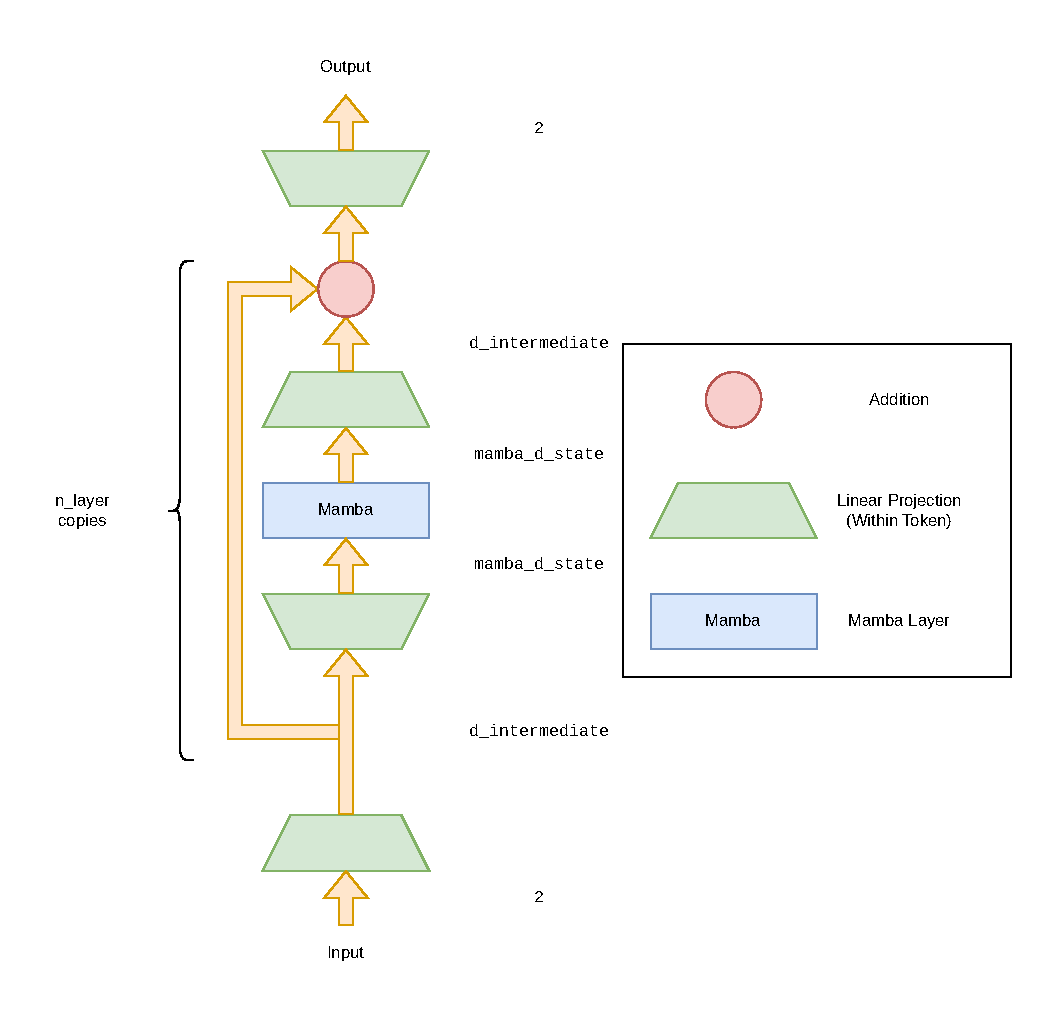
\includegraphics[width=\textwidth]{figures/sequence_stack_simple.pdf}
    \caption{Simple Mamba Stack Architecture}
    \label{simplestack}
\end{subfigure}\begin{subfigure}{0.5\textwidth}
    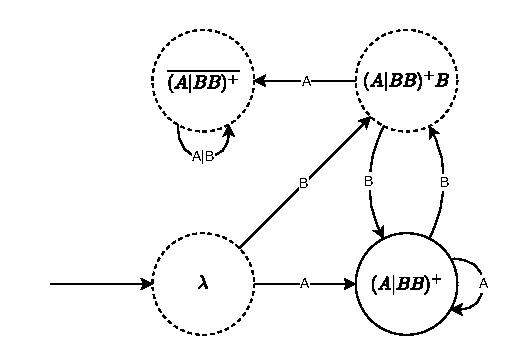
\includegraphics[width=\textwidth]{figures/a_or_bb_plus_dfa.pdf}
    \caption{DFA for \texttt{(a|bb)+}}
    \label{a_or_bb_plus_dfa}
\end{subfigure}
    \caption{}
\end{figure}

Despite their inability to perfectly predict non-star-free regular languages,
we find that Mamba is capable of recognizing certain non-star-free regular
languages with limited accuracy.

Preliminary testing on the regular language \texttt{(a|bb)+} shows a
surprisingly strong ability to recognize instances of the language, with lower
accuracy on medium-length strings.
If we construct the DFA for the language(see Figure \ref{a_or_bb_plus_dfa}), it
is clear that recognizing the language requires recognizing odd-length runs of
\verb|b|, which act as "red flags" which prevent a string from being in the
language.
We hypothesize that Mamba is searching for the most common "red flags", which
isn't enough to perfectly recognize instances of the language, but is enough
to find most instances.
If this is indeed what the model is doing, then it should achieve a nearly
perfect accuracy with member strings, since they don't contain any disqualifying
substrings, and it should struggle to get perfect accuracy with non-member
strings, since an instance might contain a disqualifying string that the model
has not learned to search for.

\textbf{Dataset} The dataset that we train Mamba to recognize is a synthetic
dataset.
The procedure for generating each instance of the dataset is as follows:
\begin{itemize}
    \item Choose a length between 1 and 64, inclusive
    \item Choose a label: either member or non-member
    \item Choose a random string that has the chosen length and label
\end{itemize}
We generate 4000 batches with 64 strings each, and train our model for 1 epoch.

\textbf{Model} The model that we train is a stack of Mamba layers with linear
projection in-between(see Figure \ref{simplestack}).
The inputs and outputs also have linear projections to make the channel numbers
match the task.
The primary hyperparameters are \verb|n_layer = 2|, \verb|mamba_d_model = 16|,
and \verb|mamba_d_state = 16|.
The rest of the hyperparameters can be found on
Github\footnote{\url{https://github.com/maxwell3025/CV-IS-Fall-2024/blob/main/mamba_formal/config/experiment_a_or_bb.yaml}}.

\textbf{Results} 
\begin{figure}
    \begin{subfigure}{0.5\textwidth}
        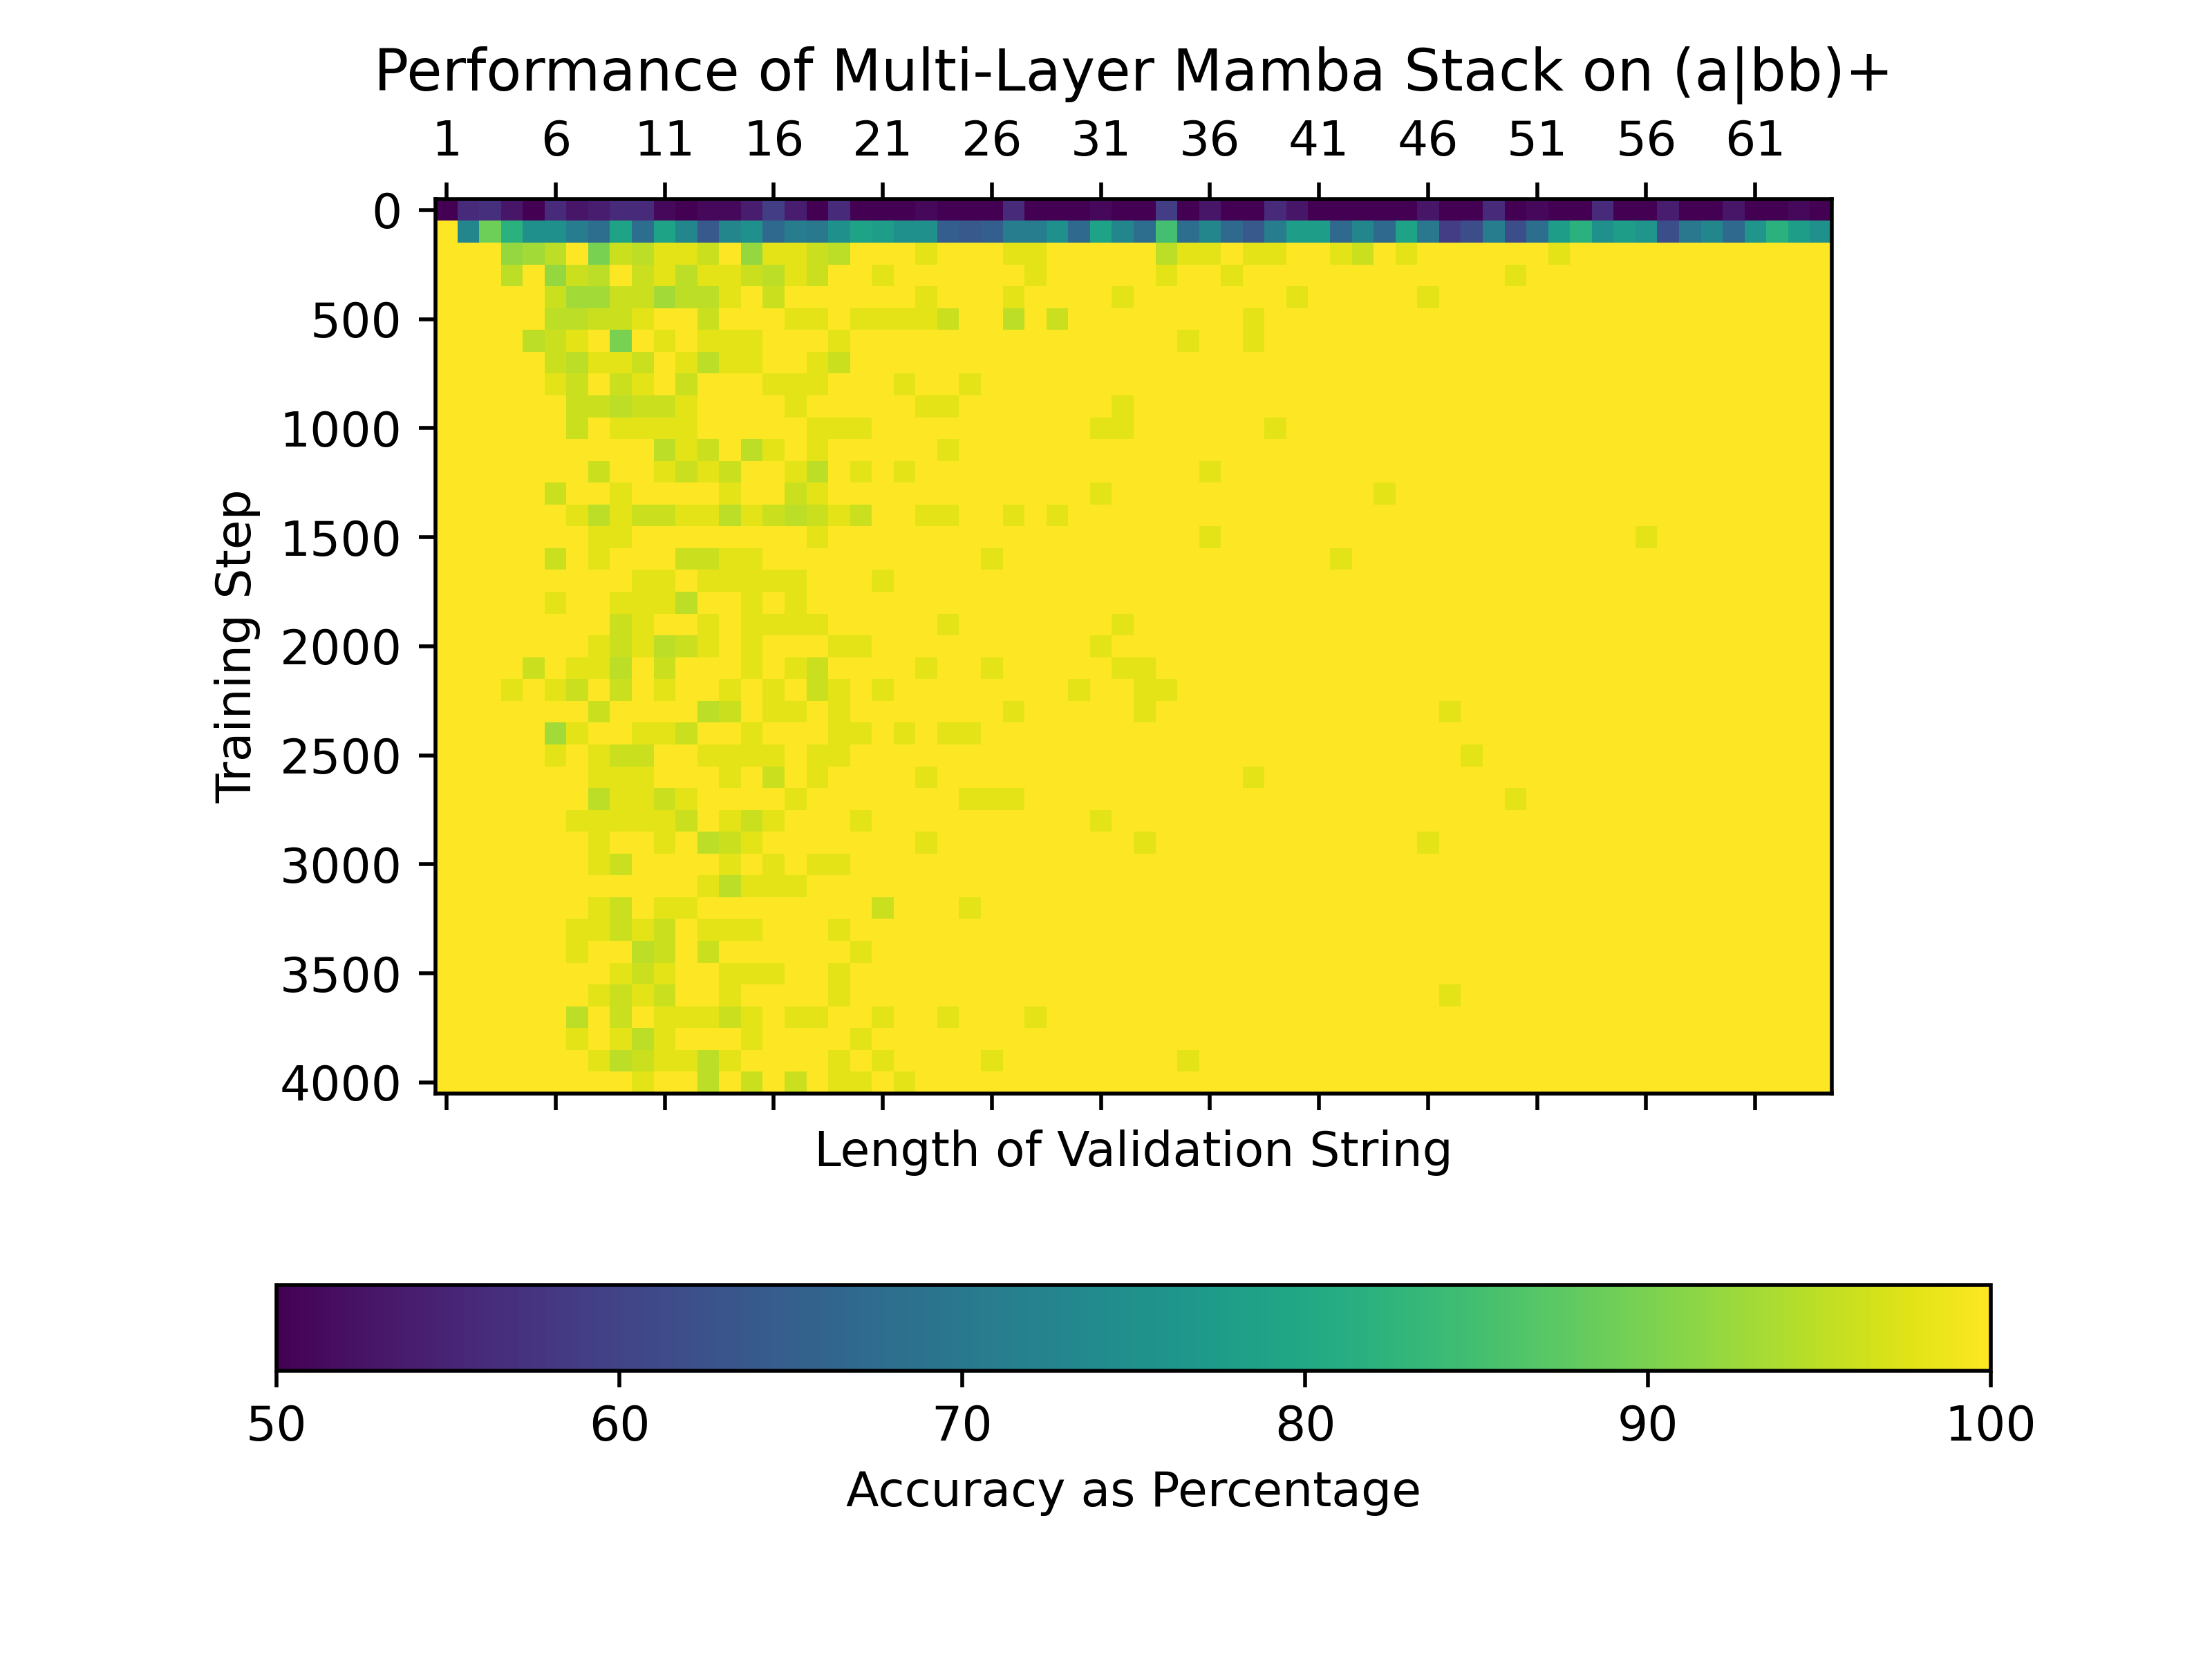
\includegraphics[width=\textwidth]{figures/a_or_bb_plus_mixed.png}
        \caption{}
    \end{subfigure}
    \begin{subfigure}{0.5\textwidth}
        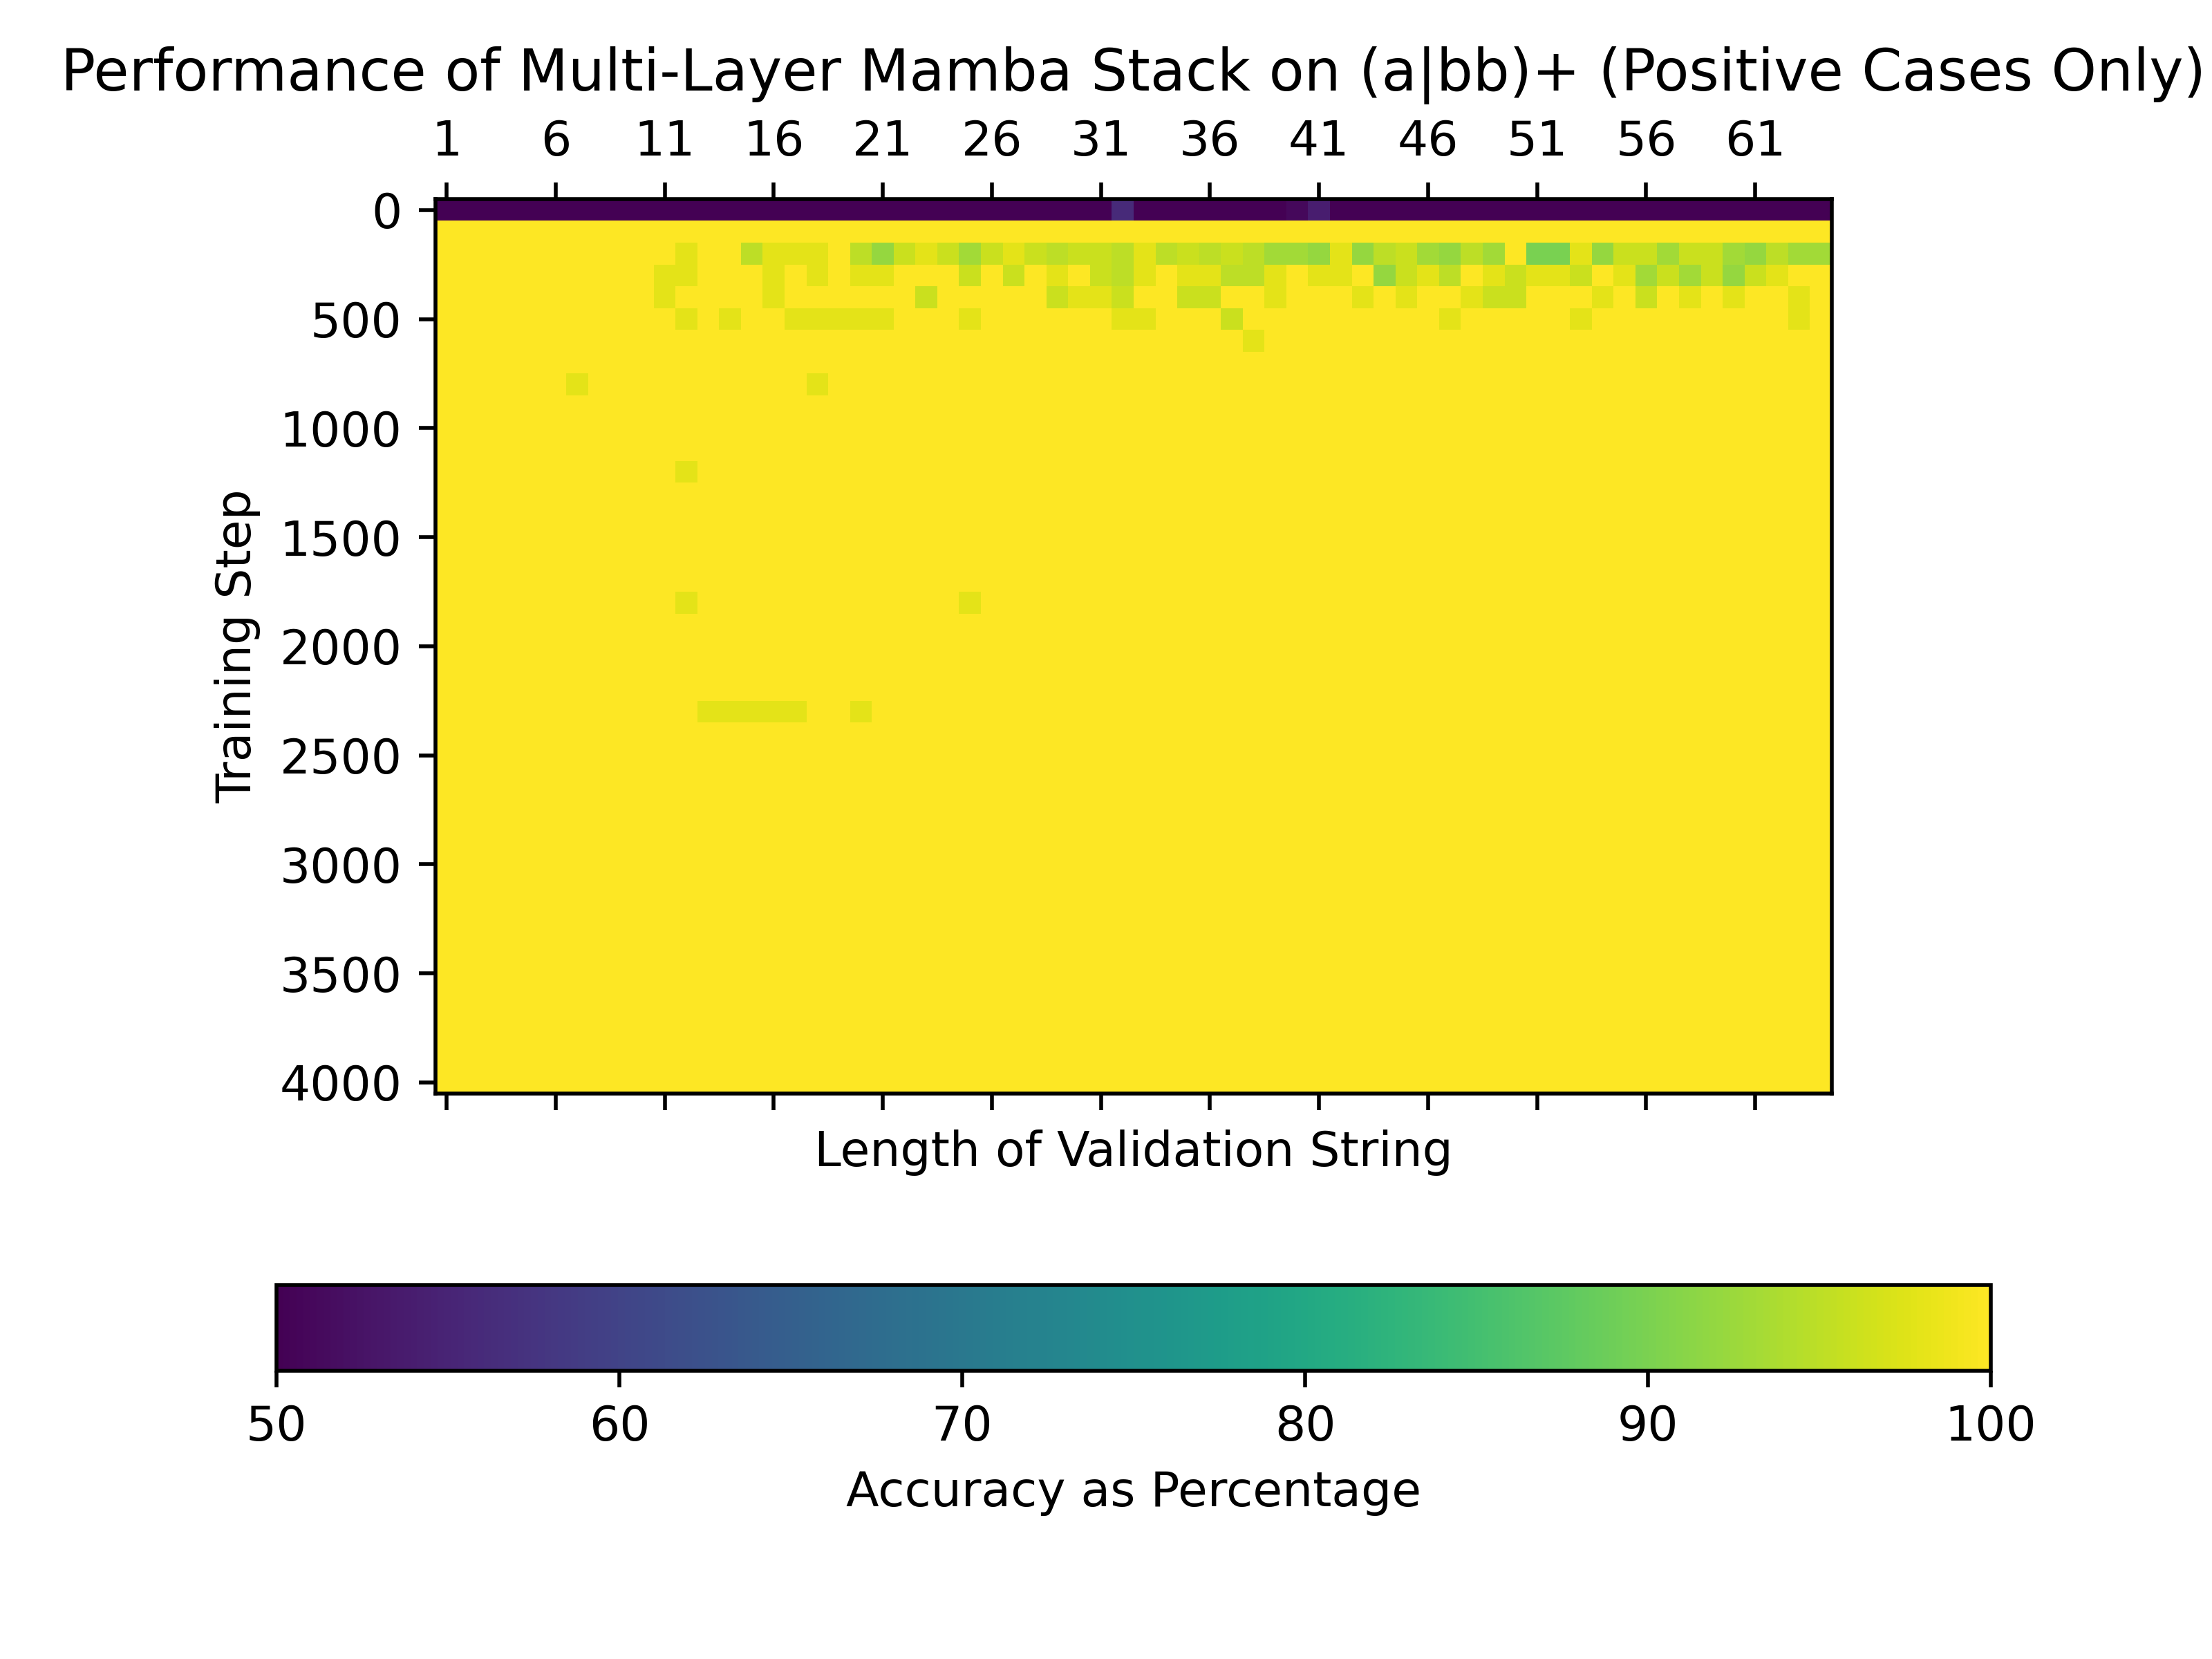
\includegraphics[width=\textwidth]{figures/a_or_bb_plus_positive_only.png}
        \caption{}
    \end{subfigure}
    \caption{Results for \texttt{a|bb+}}
\end{figure}
We find that the model quickly attains nearly perfect performance on positive
cases, with the trained model only making errors with negative cases.
This strongly suggests that our hypothesis is true.
The model is correctly identifying that positive cases lack the forbidden
strings that the model memorized, and the model is failing to recognize some
negative cases, since they contain odd-length forbidden strings that were not
memorized.

\subsection{Formation of "Bad Habits" with Mamba}
Given Mamba's limited ability to recognize regular languages, it would be useful
to place it alongside more formally powerful models such as LSTMs, which can
trivially model general regular languages given large enough
parameters\cite{lstmformal}. Unfortunately, preliminary testing found that the
inclusion of Mamba in series with LSTMs leads to a degradation of generalization
ability.

In the literature, we find that machine learning architectures like
MedMamba\cite{medmamba}, VMamba\cite{vmamba}, and MambaND\cite{mamband} apply
drop-path to the output of Mamba layers.
Drop-path is a normalization layer introduced by FractalNet\cite{fractalnet} in
which the outputs of entire layers in an architecture are set to zero.
As stated by the authors, this causes the model to learn how to do the task
without using certain layers.
We suspect that drop-path is included in Mamba-based architectures since Mamba
learns incorrect approximations of various tasks, which override the correct
solutions learned by other layers.
Drop-path then trains the other layers to learn their own(correct) solutions.
In order to confirm these findings, we test a mixed Mamba model to solve a task
that Mamba alone cannot solve.

It has been shown that Mamba cannot recognize even bitstrings\cite{ssmformal},
a finding we confirm in our own preliminary testing, while LSTM has been shown
to trivially solve this task. Thus, we proceed with the following experiment:

\textbf{Model} Our model in this test is identical to the model shown in
Figure \ref{simplestack}, with the change that 2 input layers are replaced with
LSTM layers.
In addition, drop path layers are placed after each Mamba layer depending on
the experimental group.

\textbf{Dataset}
The dataset that we use is exactly the same as the one used in the previous
experiment, except that instead of sampling the language \texttt{a|bb+},
we sample the language \texttt{(0*10*10*)*}, or the language of even bitstrings.

\textbf{Results}
\begin{figure}
    \begin{subfigure}{0.5\textwidth}
        \begin{center}
        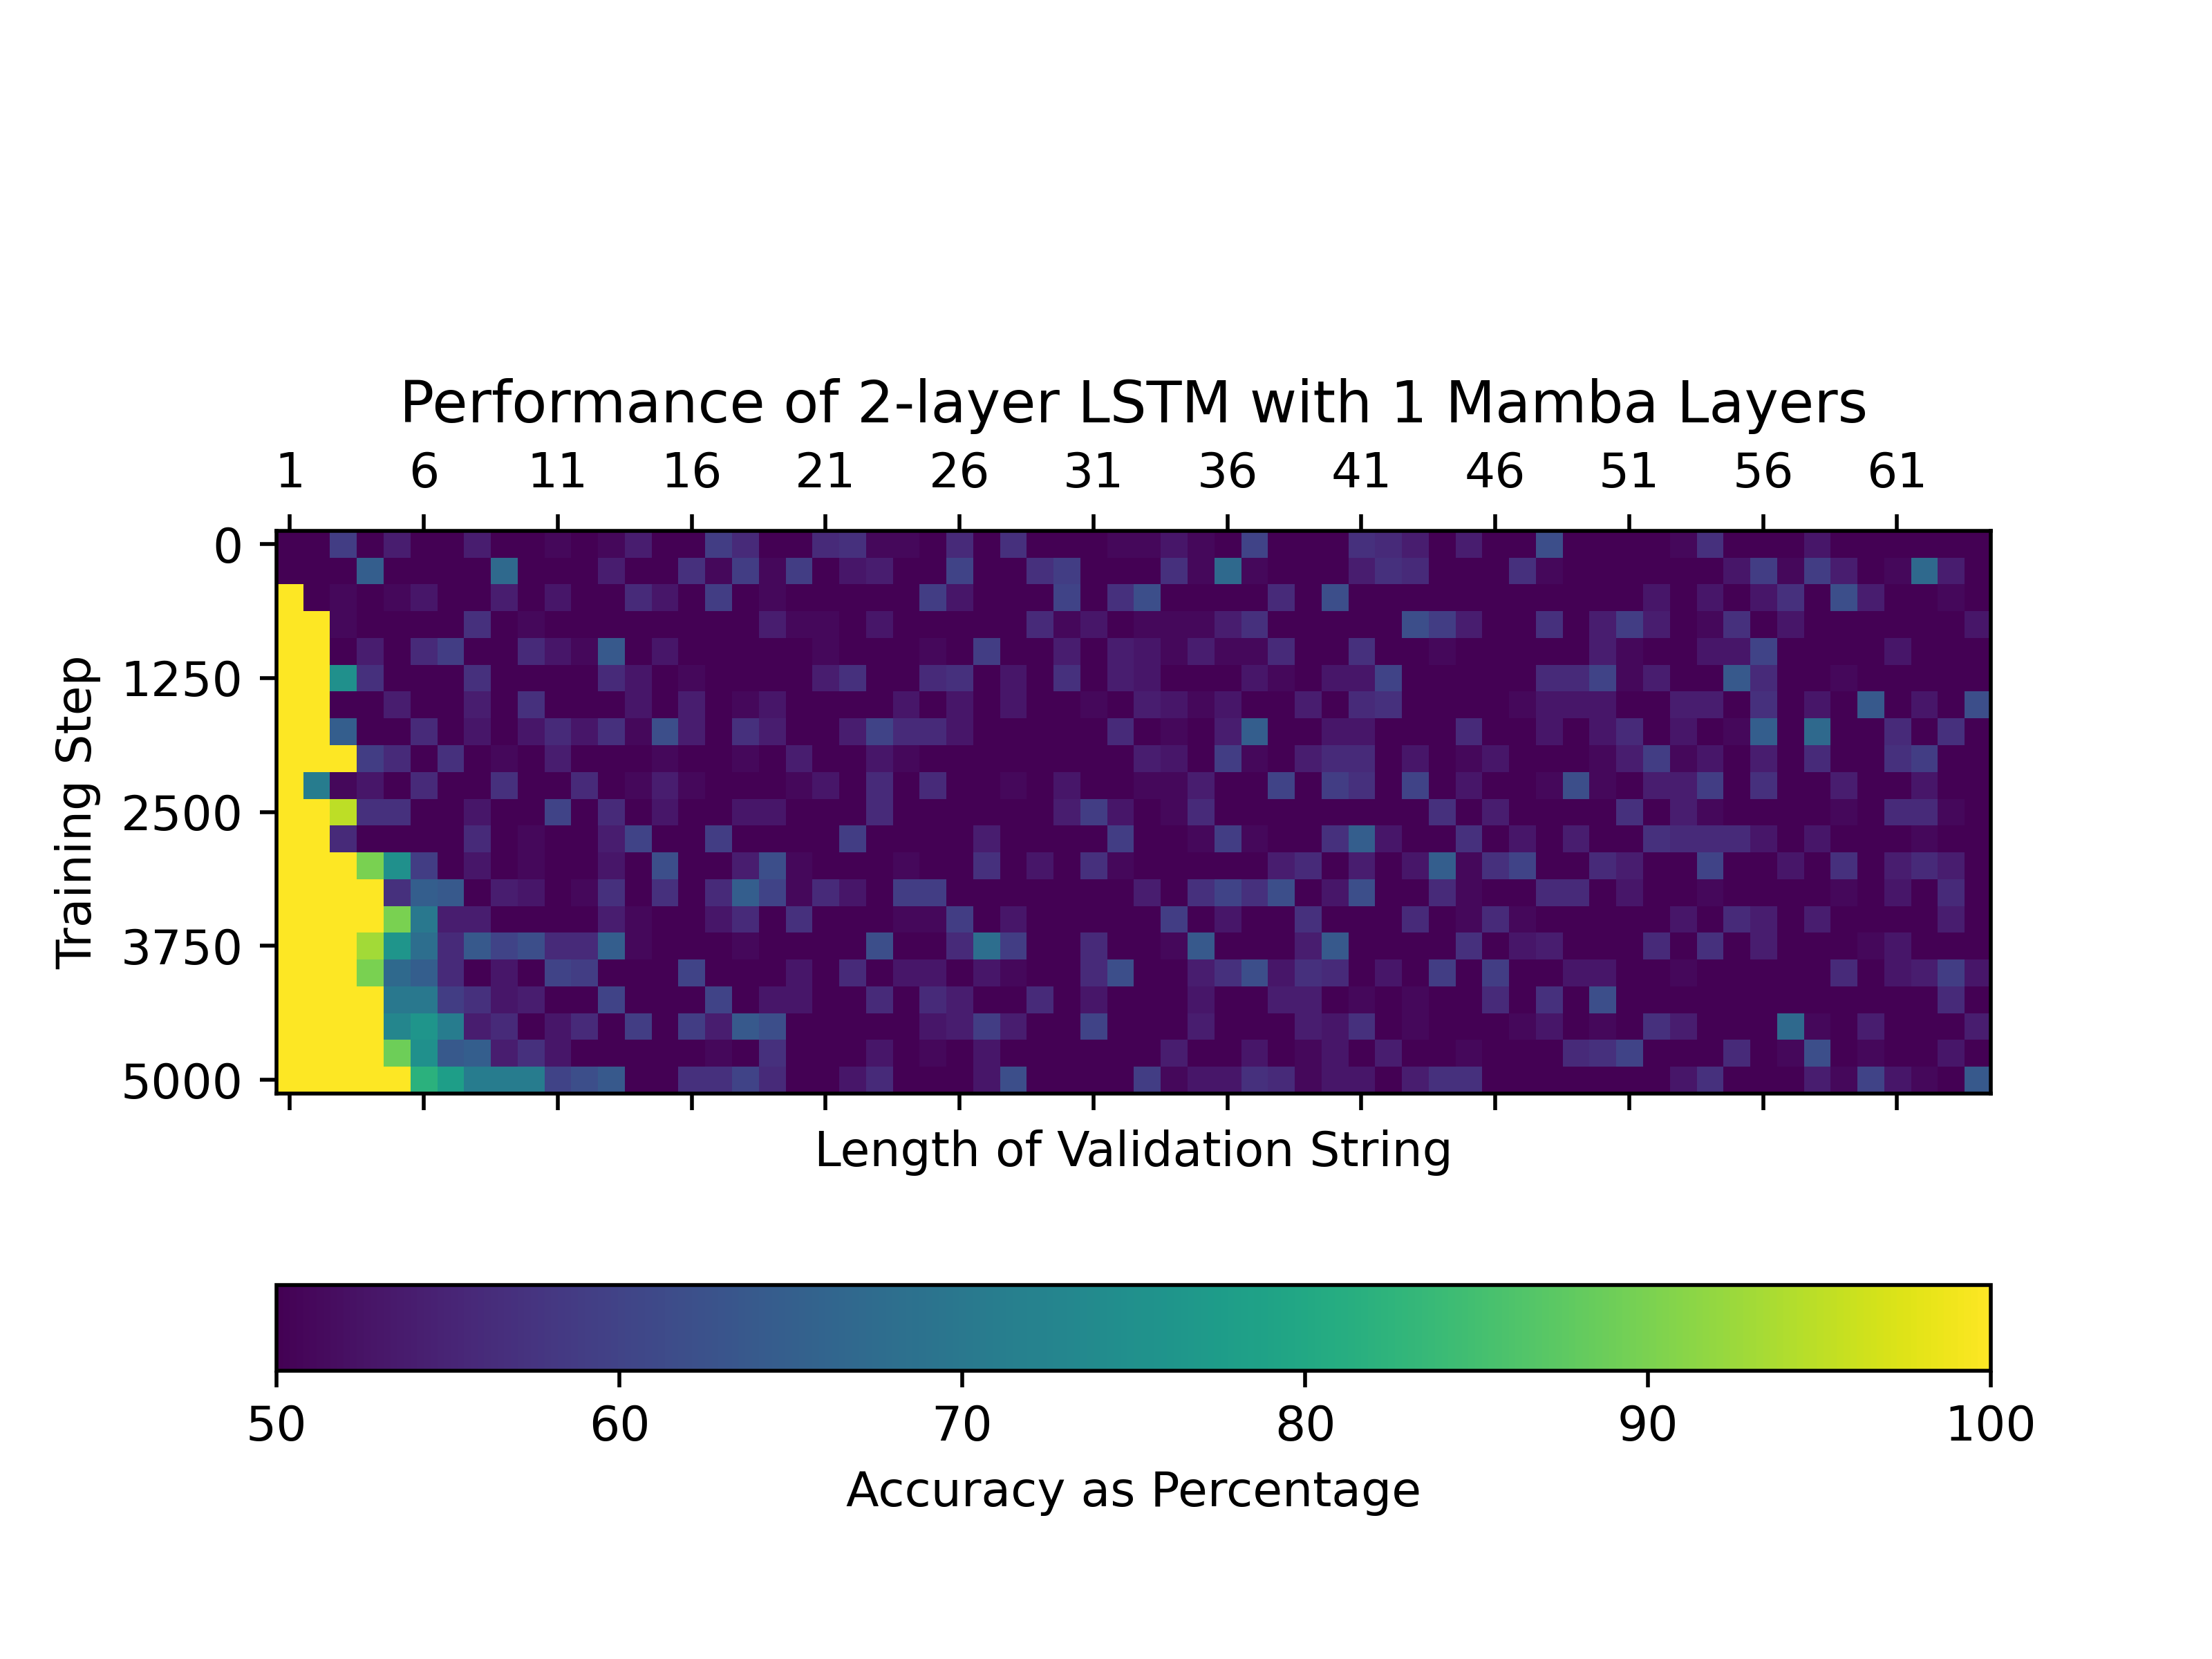
\includegraphics[width=0.8\textwidth]{figures/parity_lstm_False_3_1.png}
        \end{center}
    \end{subfigure}\begin{subfigure}{0.5\textwidth}
        \begin{center}
        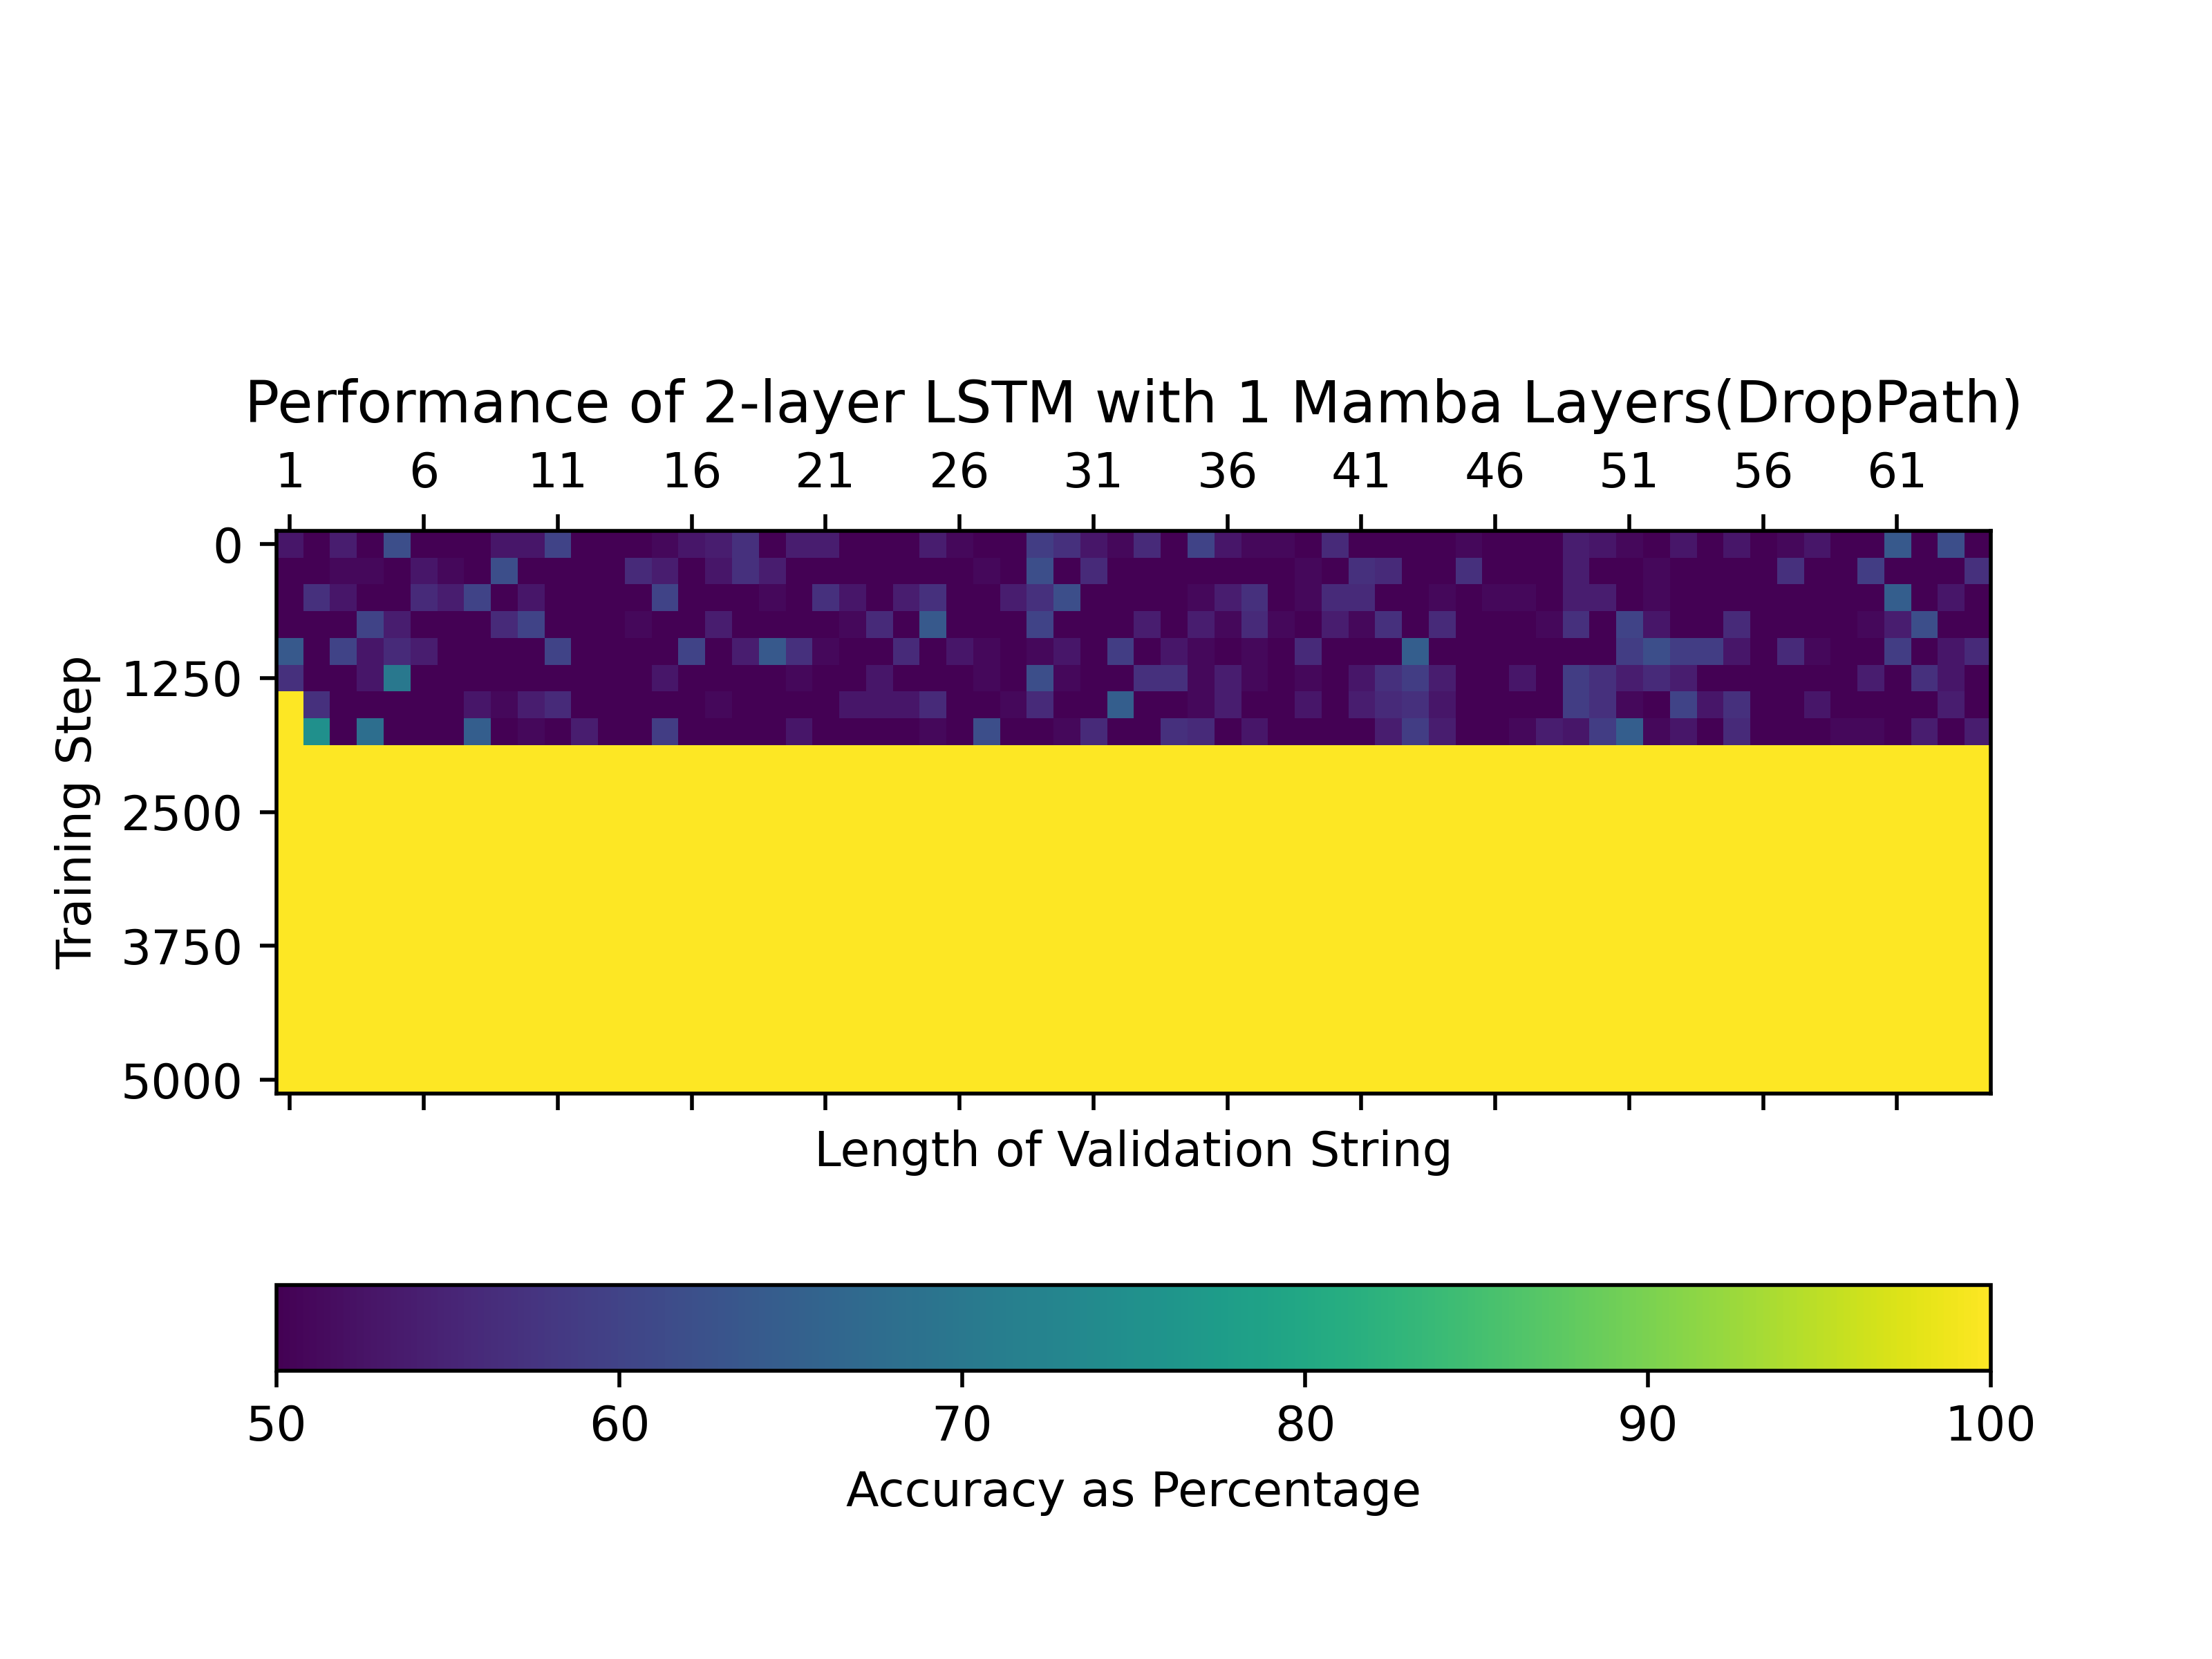
\includegraphics[width=0.8\textwidth]{figures/parity_lstm_True_3_1.png}
        \end{center}
    \end{subfigure}
    \begin{subfigure}{0.5\textwidth}
        \begin{center}
        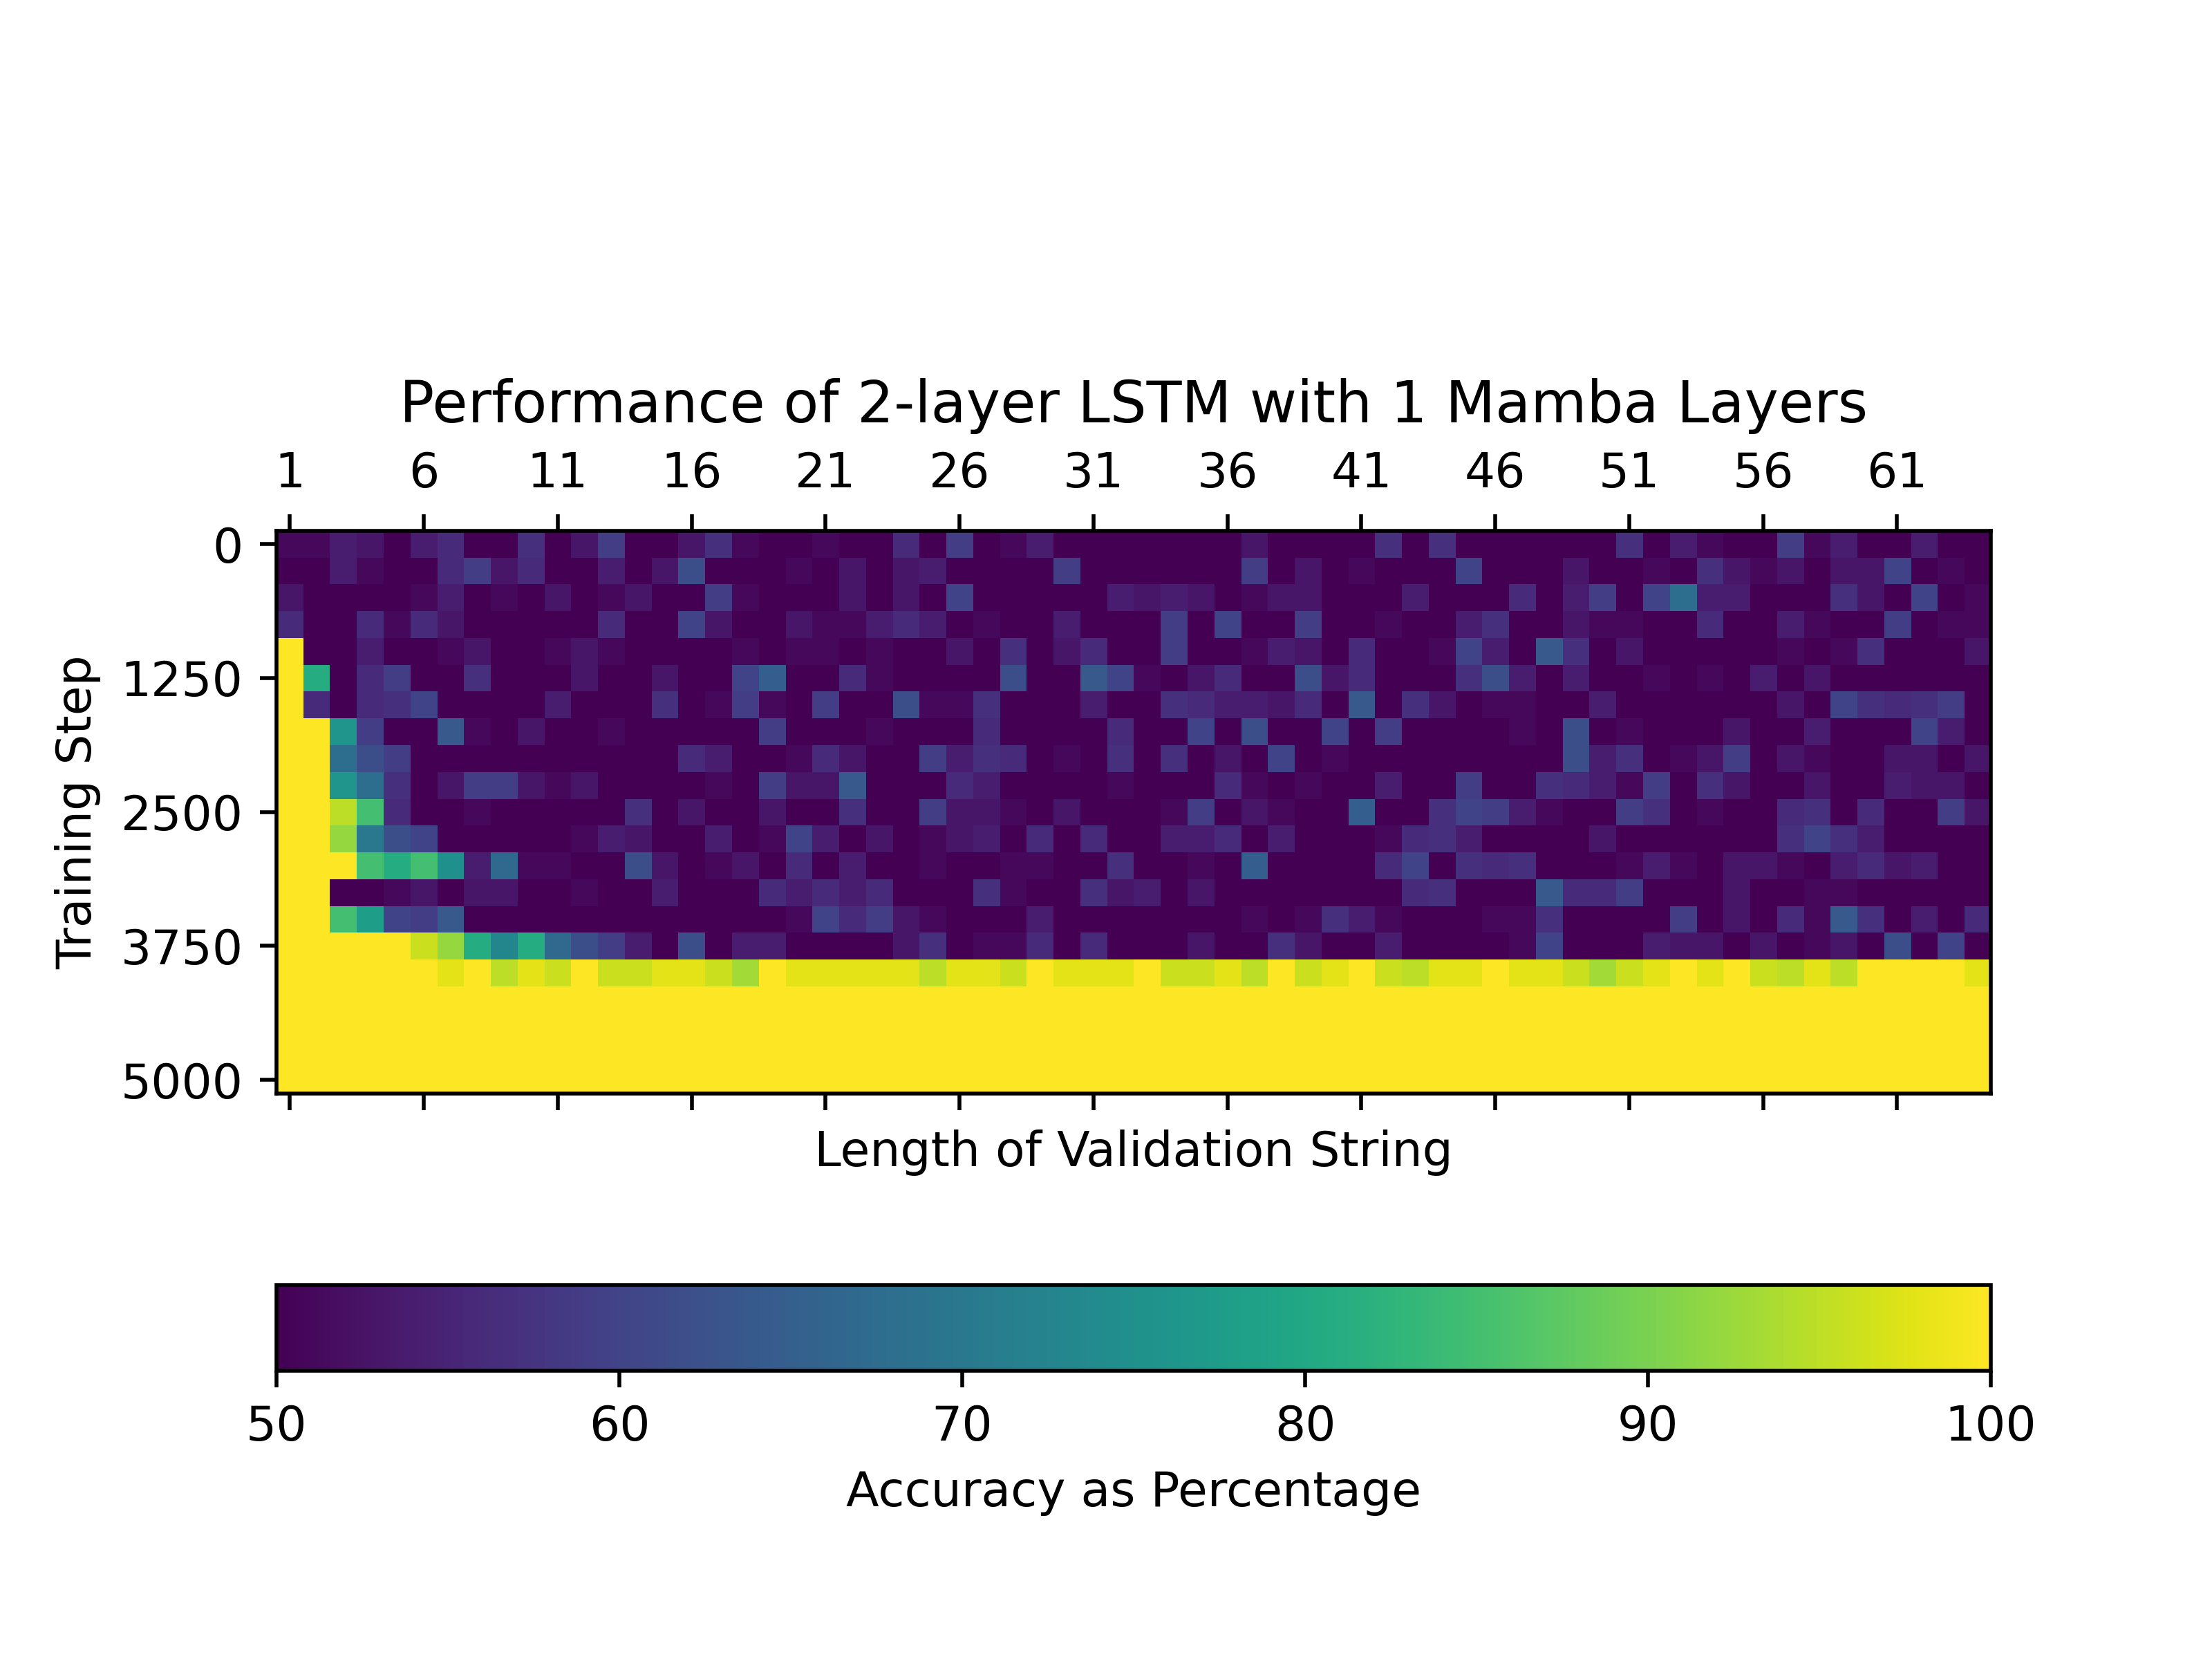
\includegraphics[width=0.8\textwidth]{figures/parity_lstm_False_3_2.png}
        \end{center}
    \end{subfigure}\begin{subfigure}{0.5\textwidth}
        \begin{center}
        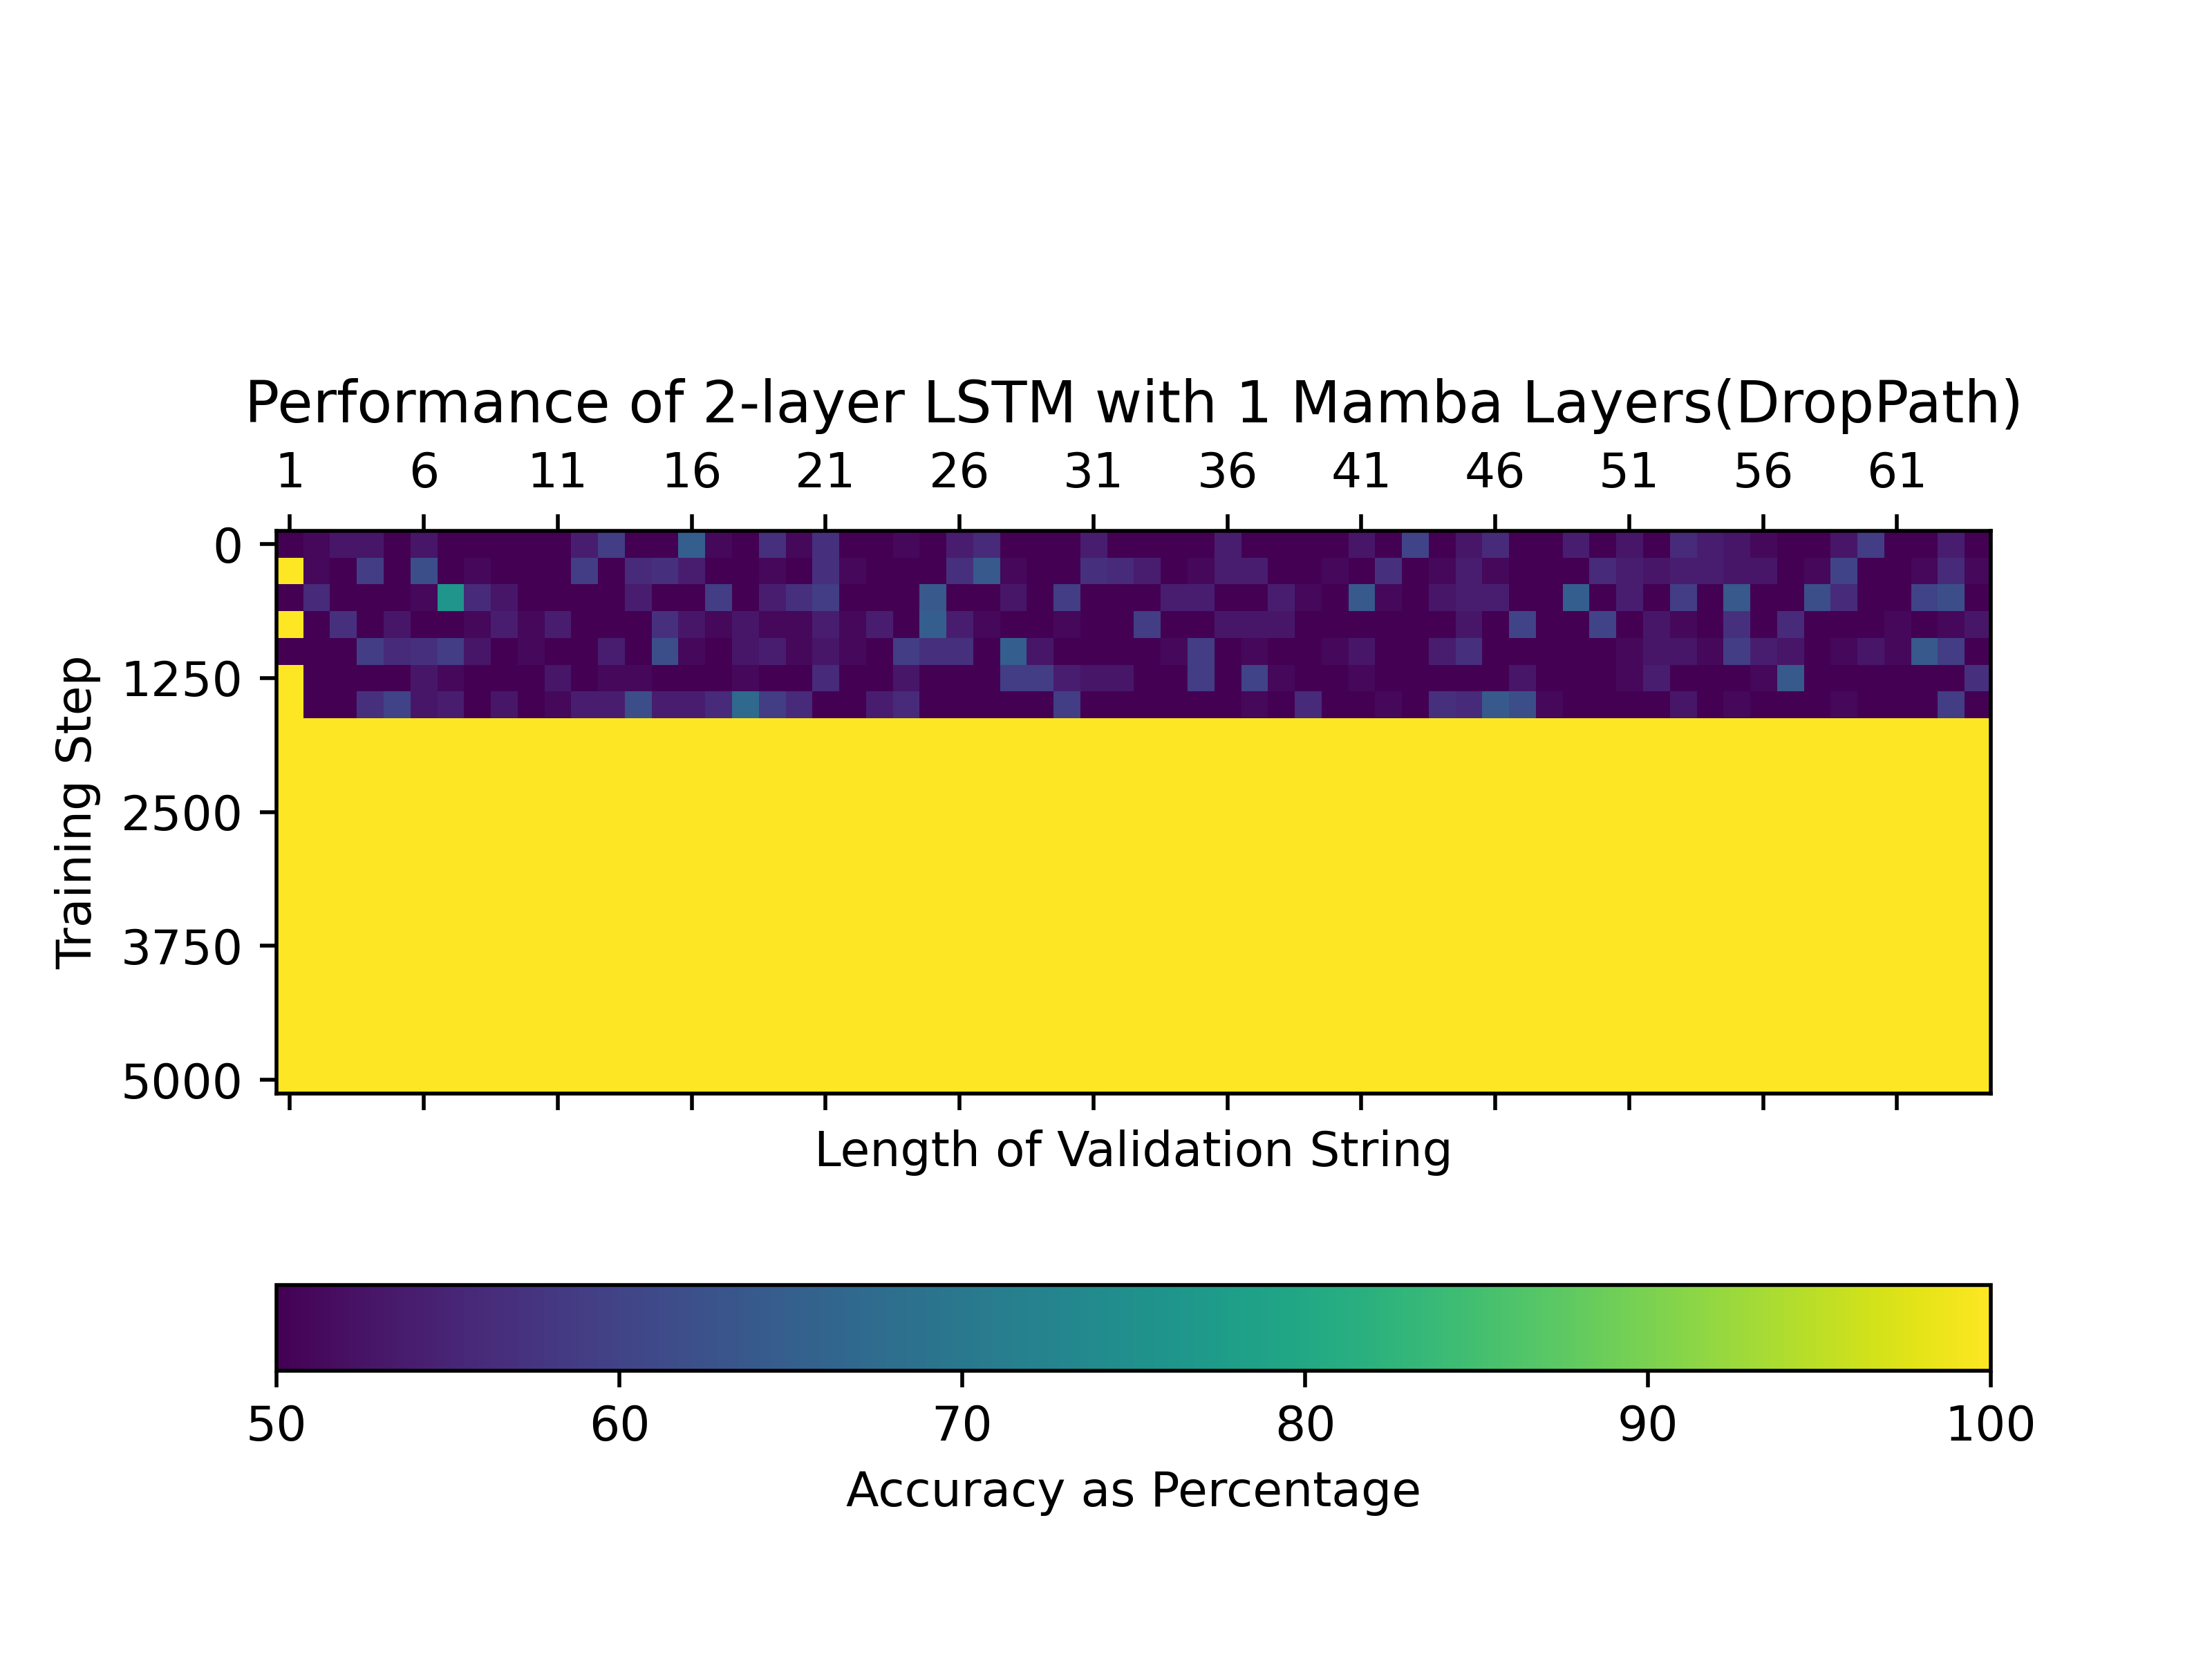
\includegraphics[width=0.8\textwidth]{figures/parity_lstm_True_3_2.png}
        \end{center}
    \end{subfigure}
    \begin{subfigure}{0.5\textwidth}
        \begin{center}
        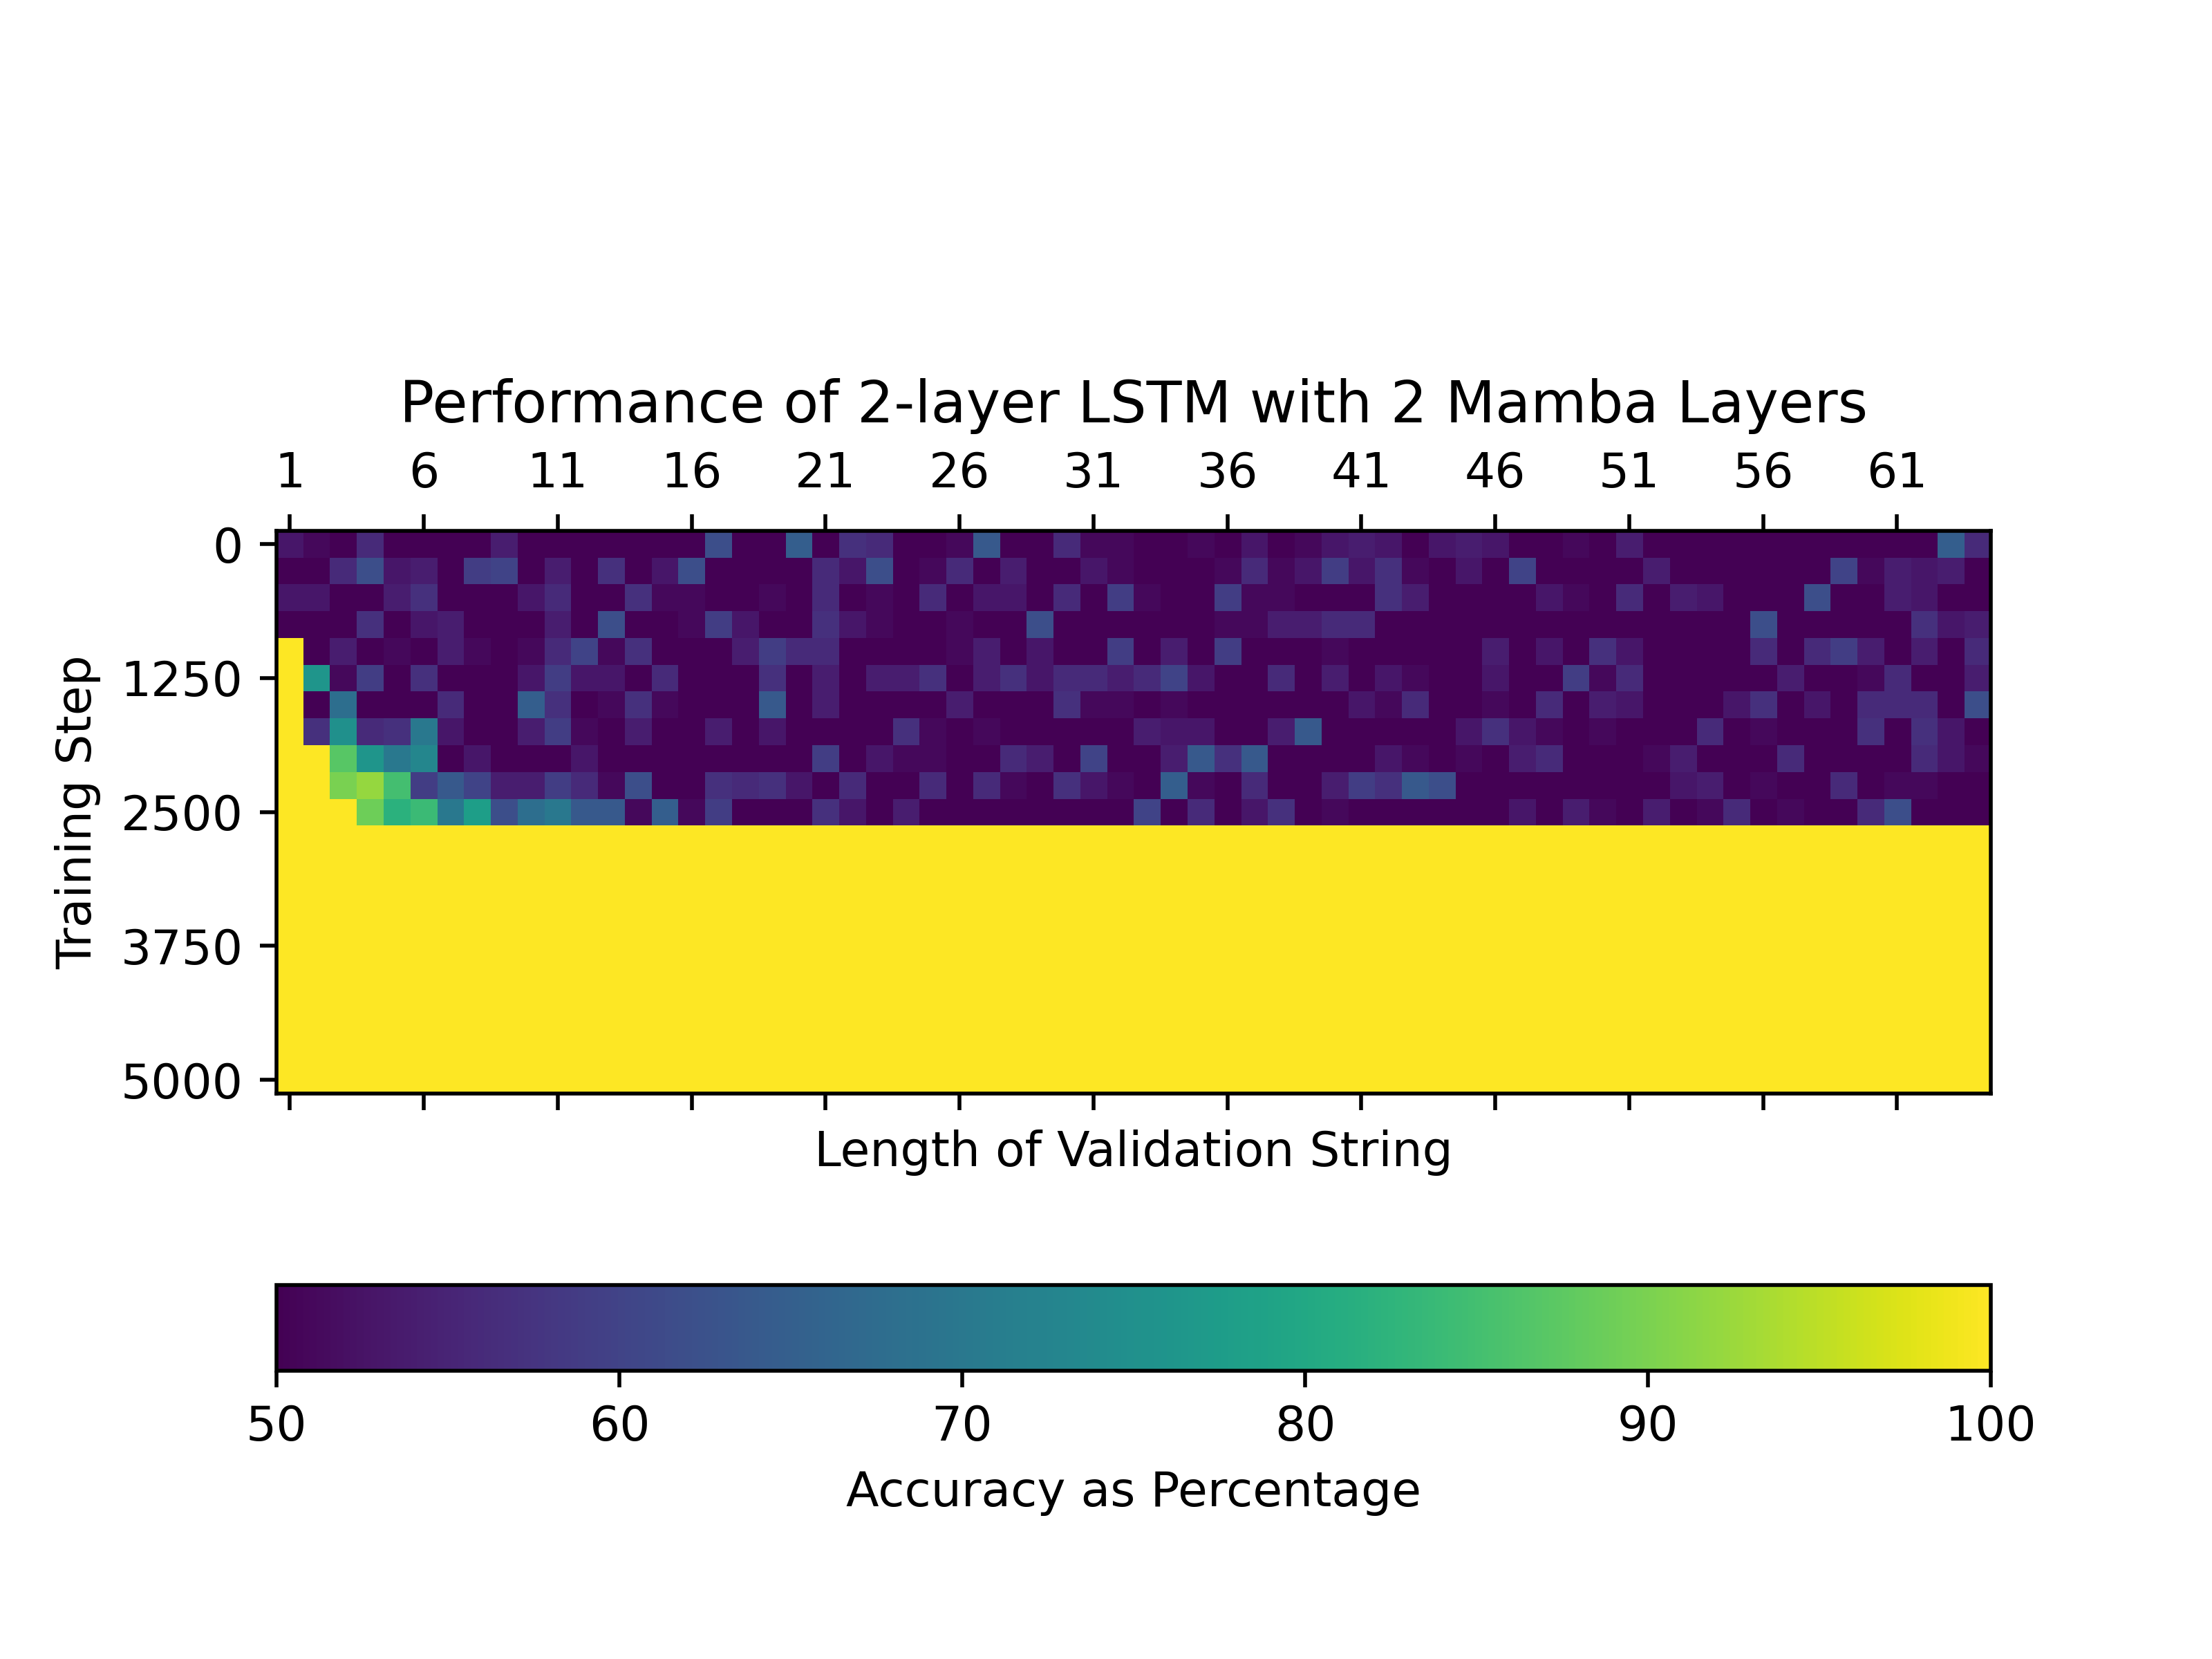
\includegraphics[width=0.8\textwidth]{figures/parity_lstm_False_4_1.png}
        \end{center}
    \end{subfigure}\begin{subfigure}{0.5\textwidth}
        \begin{center}
        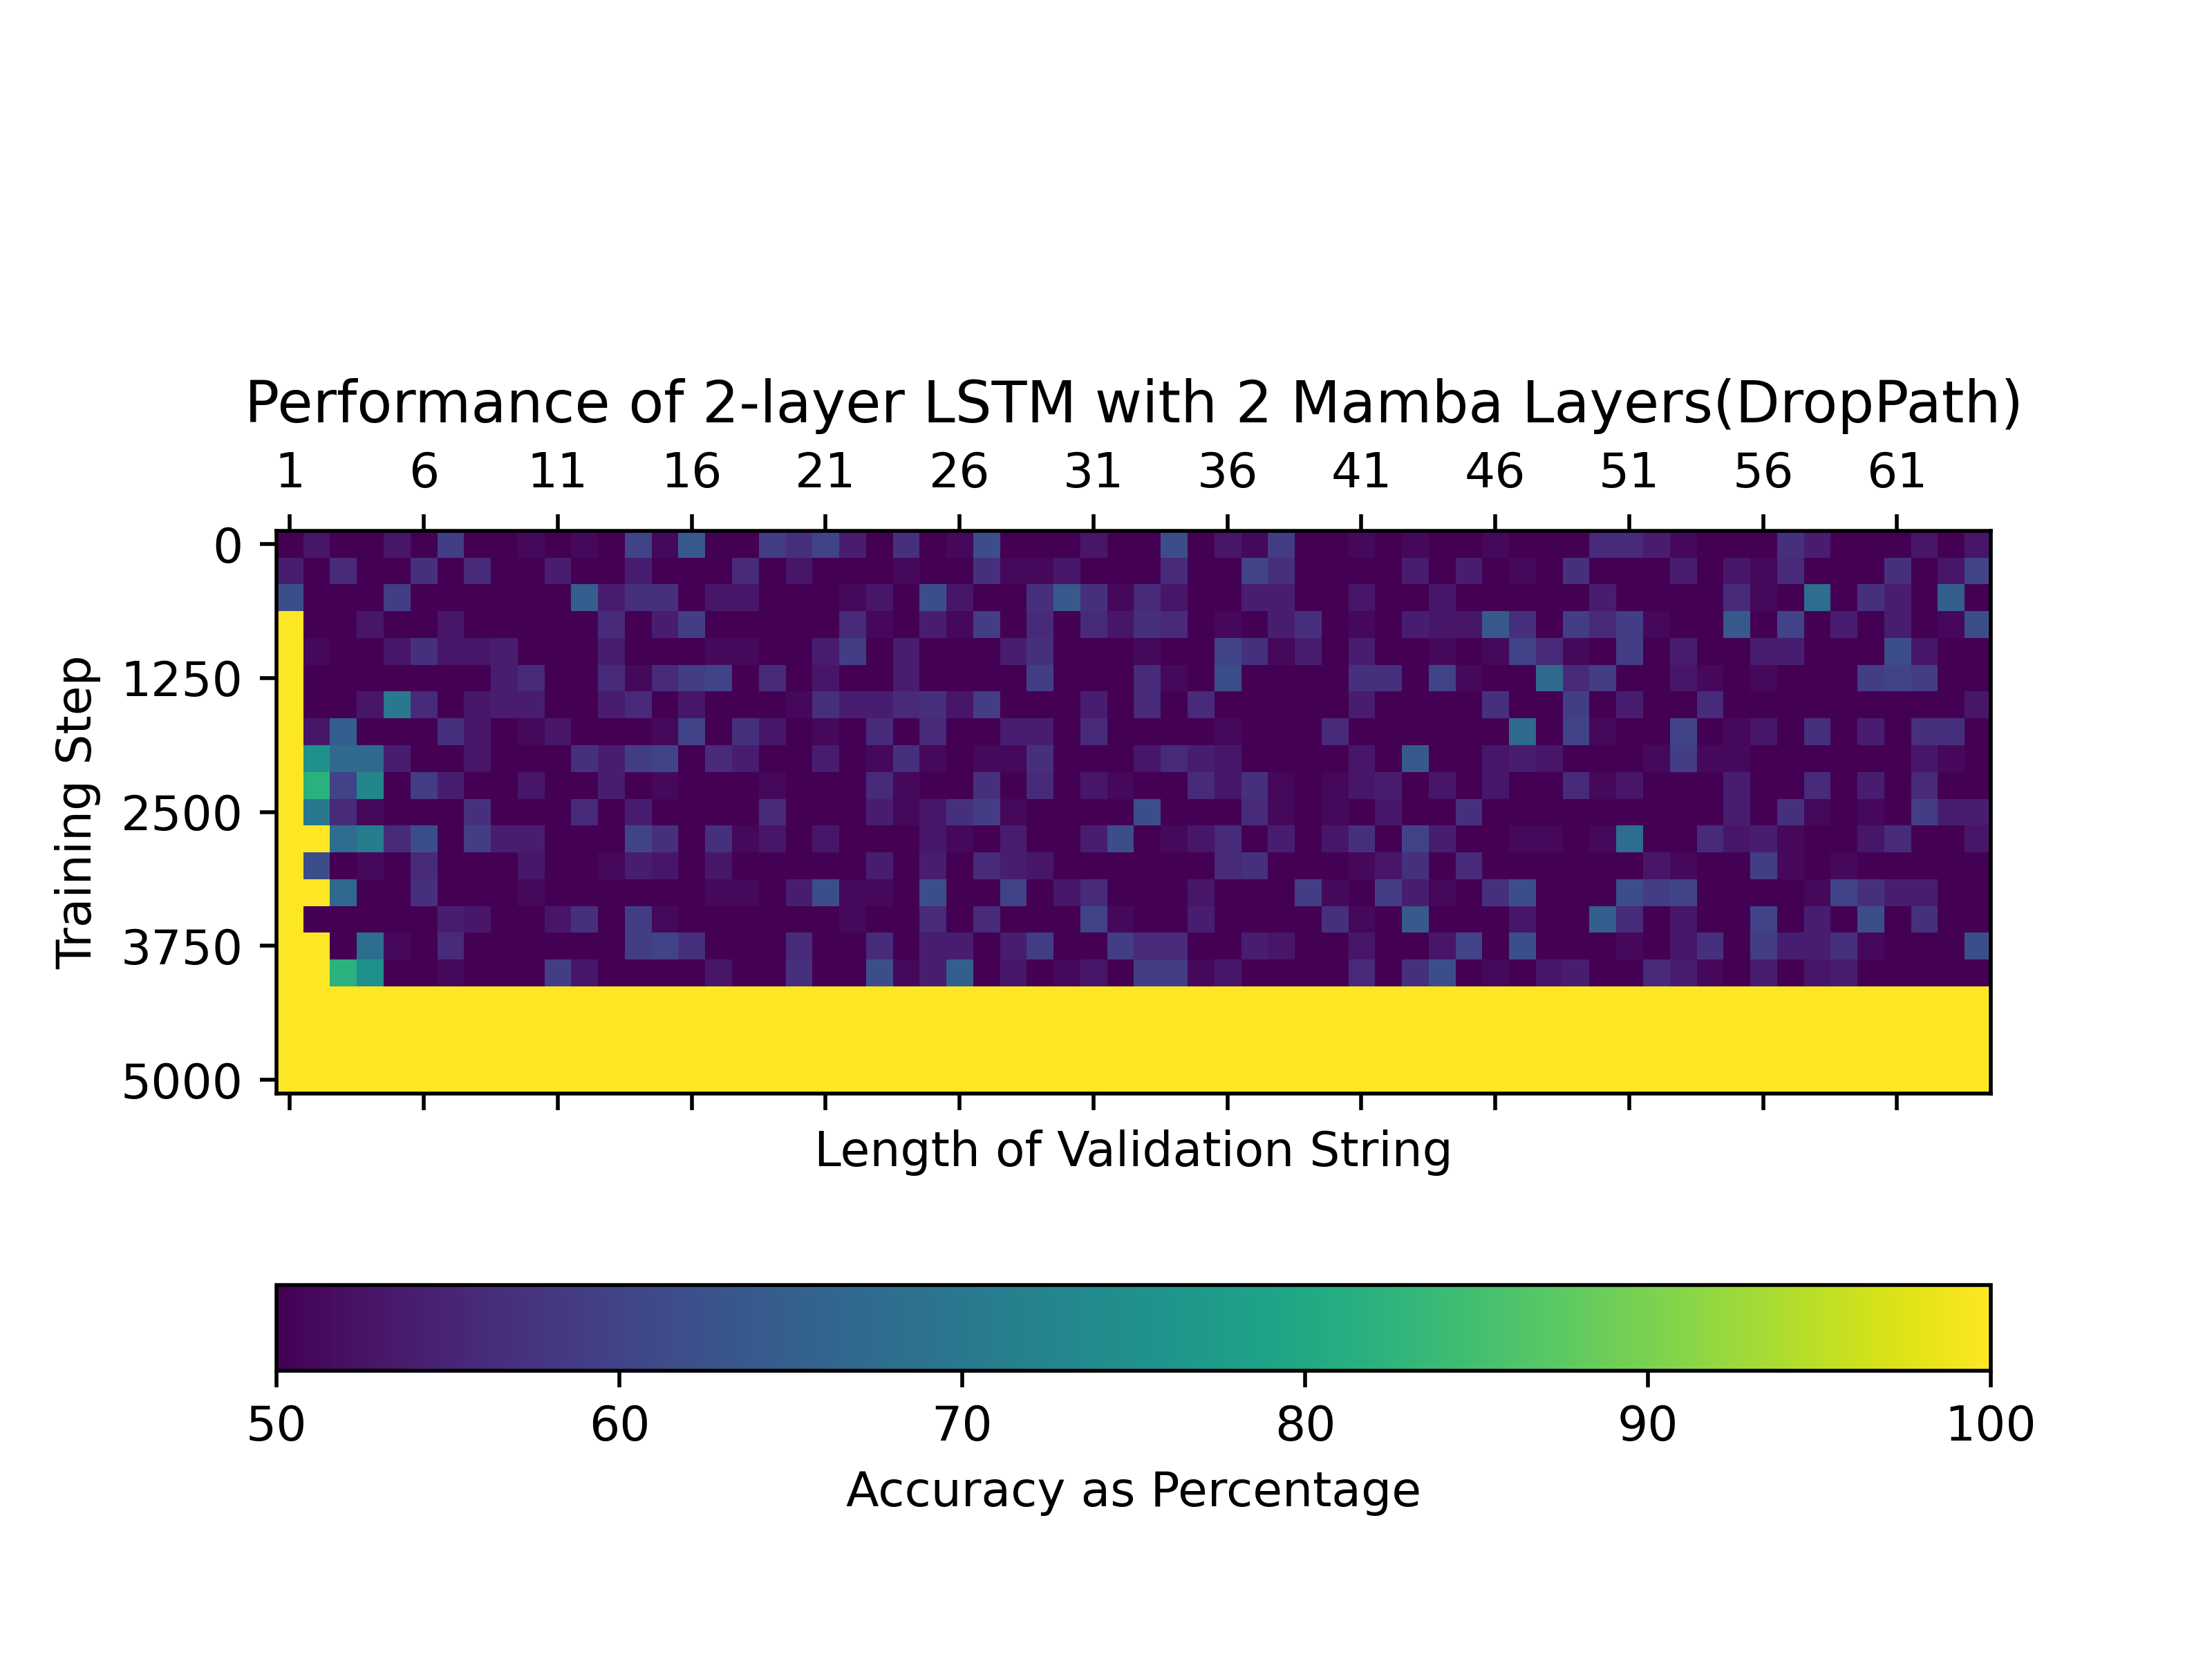
\includegraphics[width=0.8\textwidth]{figures/parity_lstm_True_4_1.png}
        \end{center}
    \end{subfigure}
    \begin{subfigure}{0.5\textwidth}
        \begin{center}
        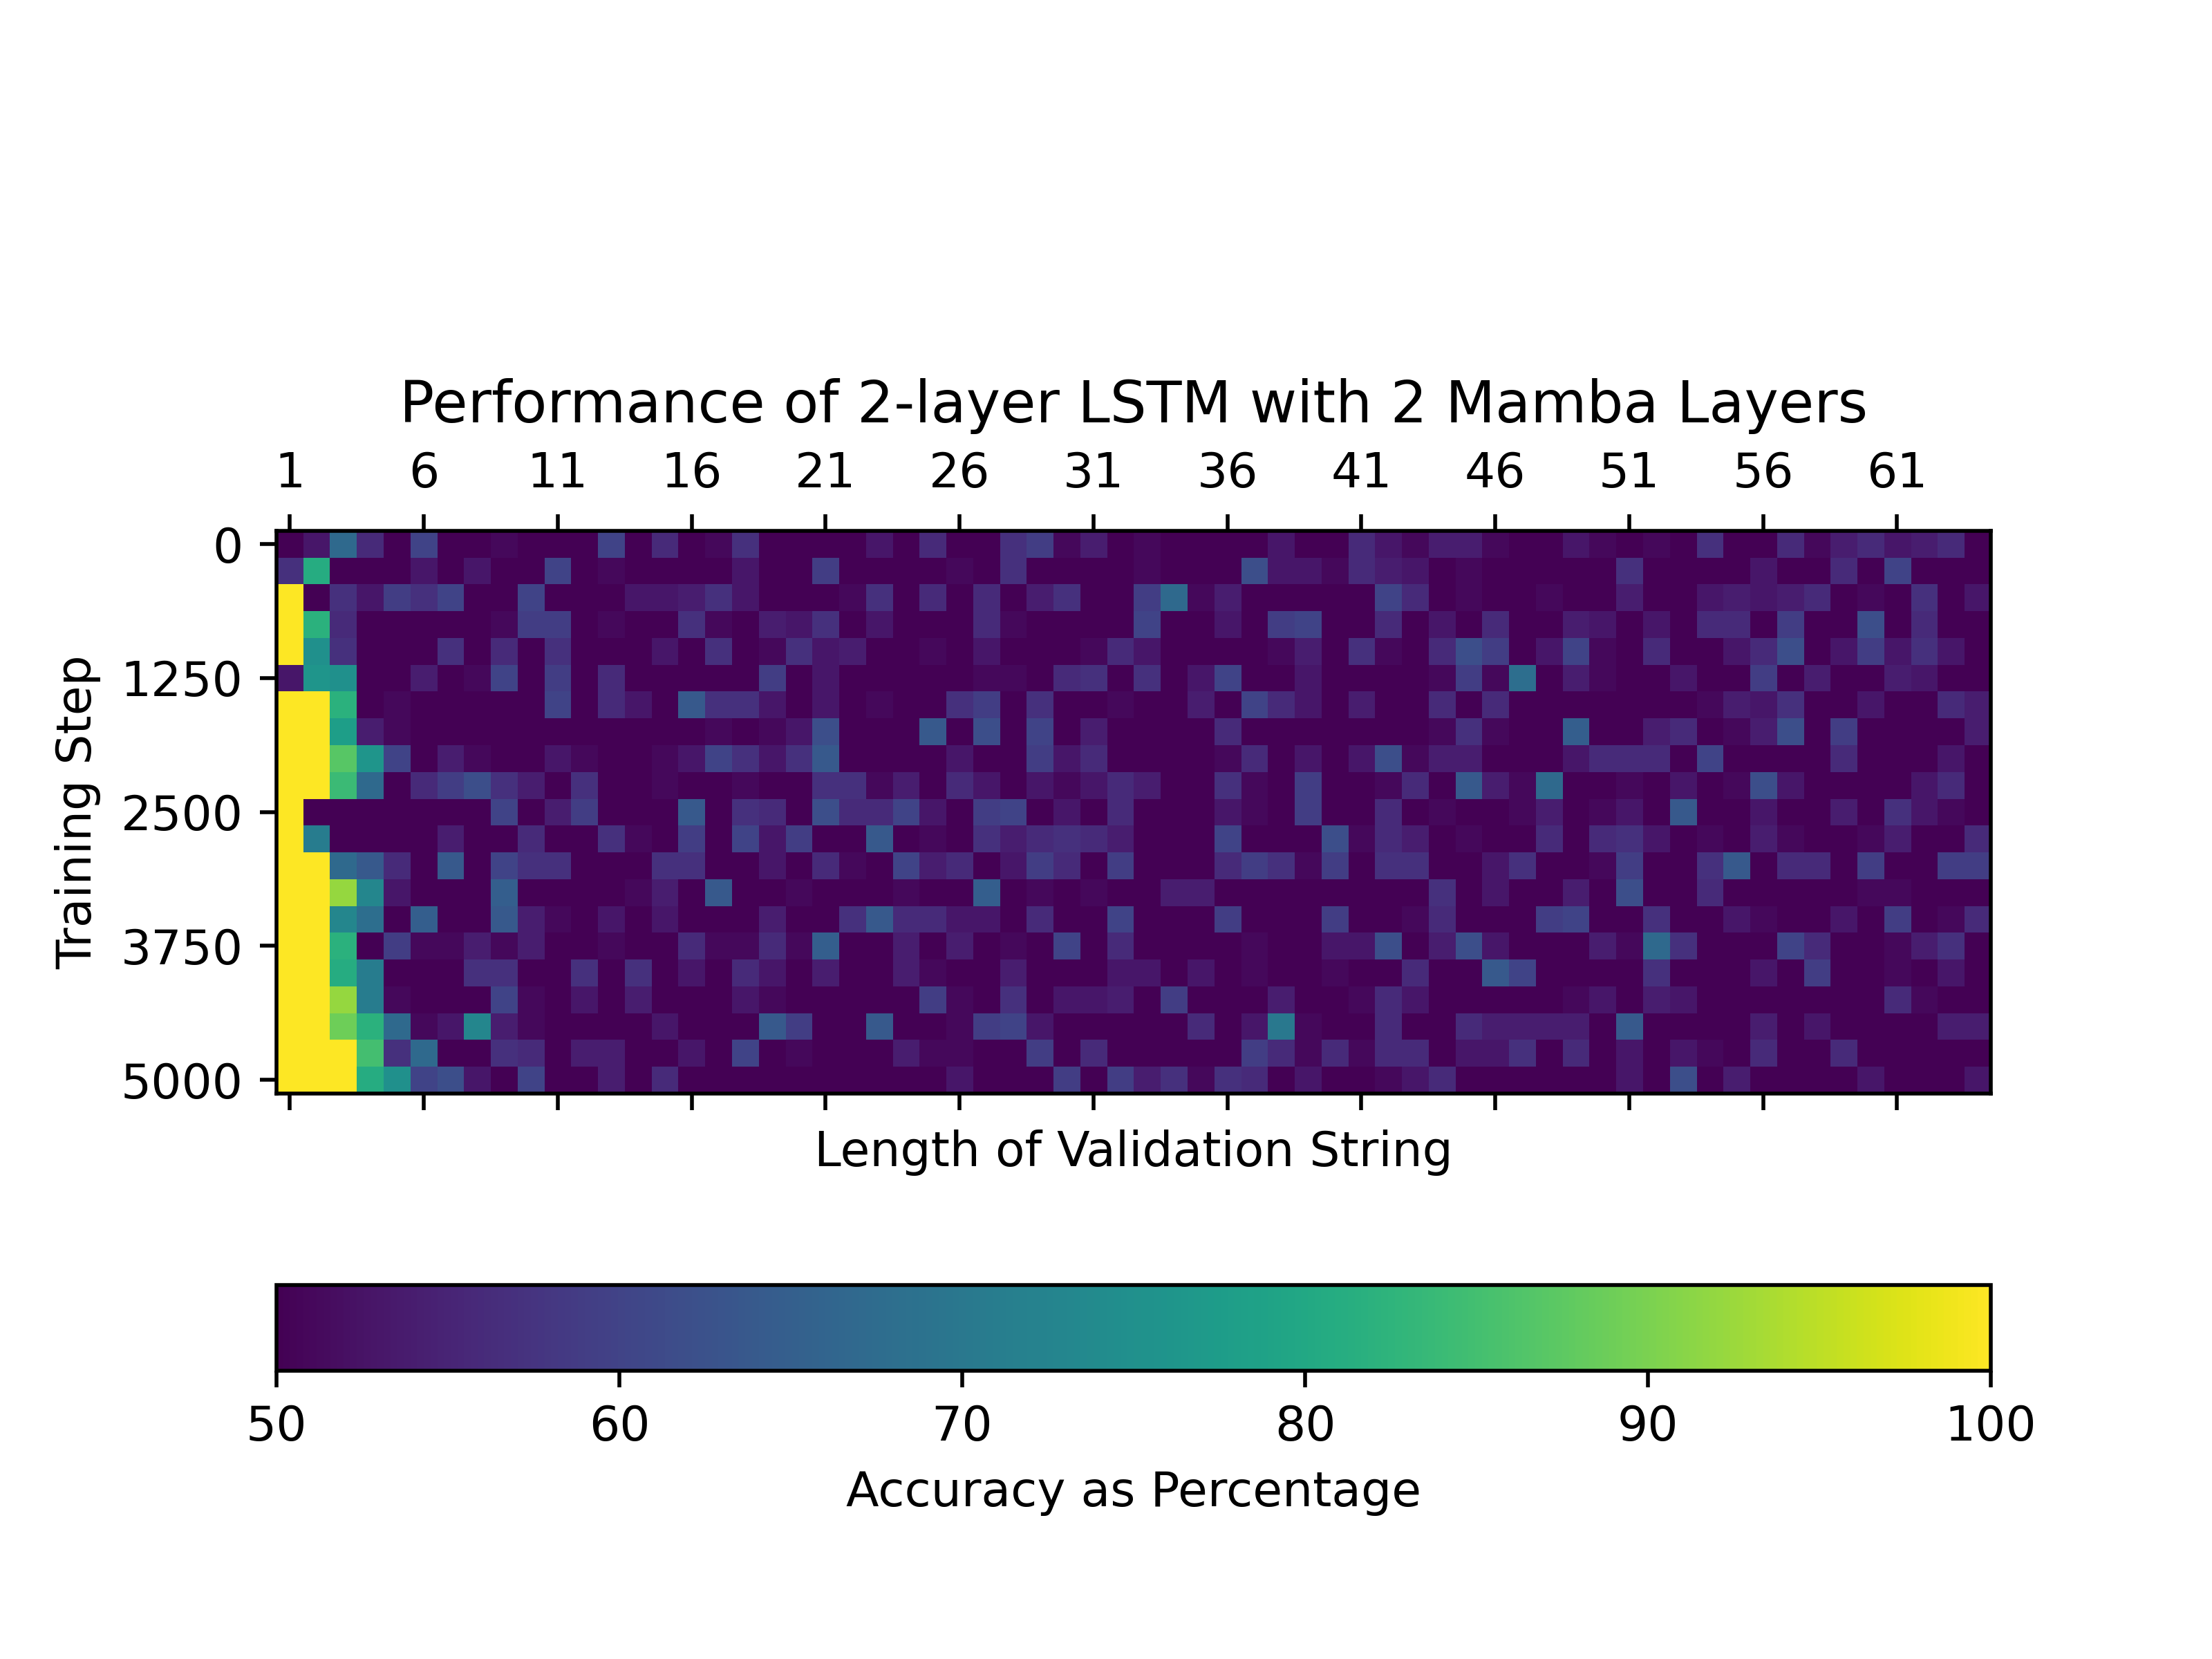
\includegraphics[width=0.8\textwidth]{figures/parity_lstm_False_4_2.png}
        \end{center}
    \end{subfigure}\begin{subfigure}{0.5\textwidth}
        \begin{center}
        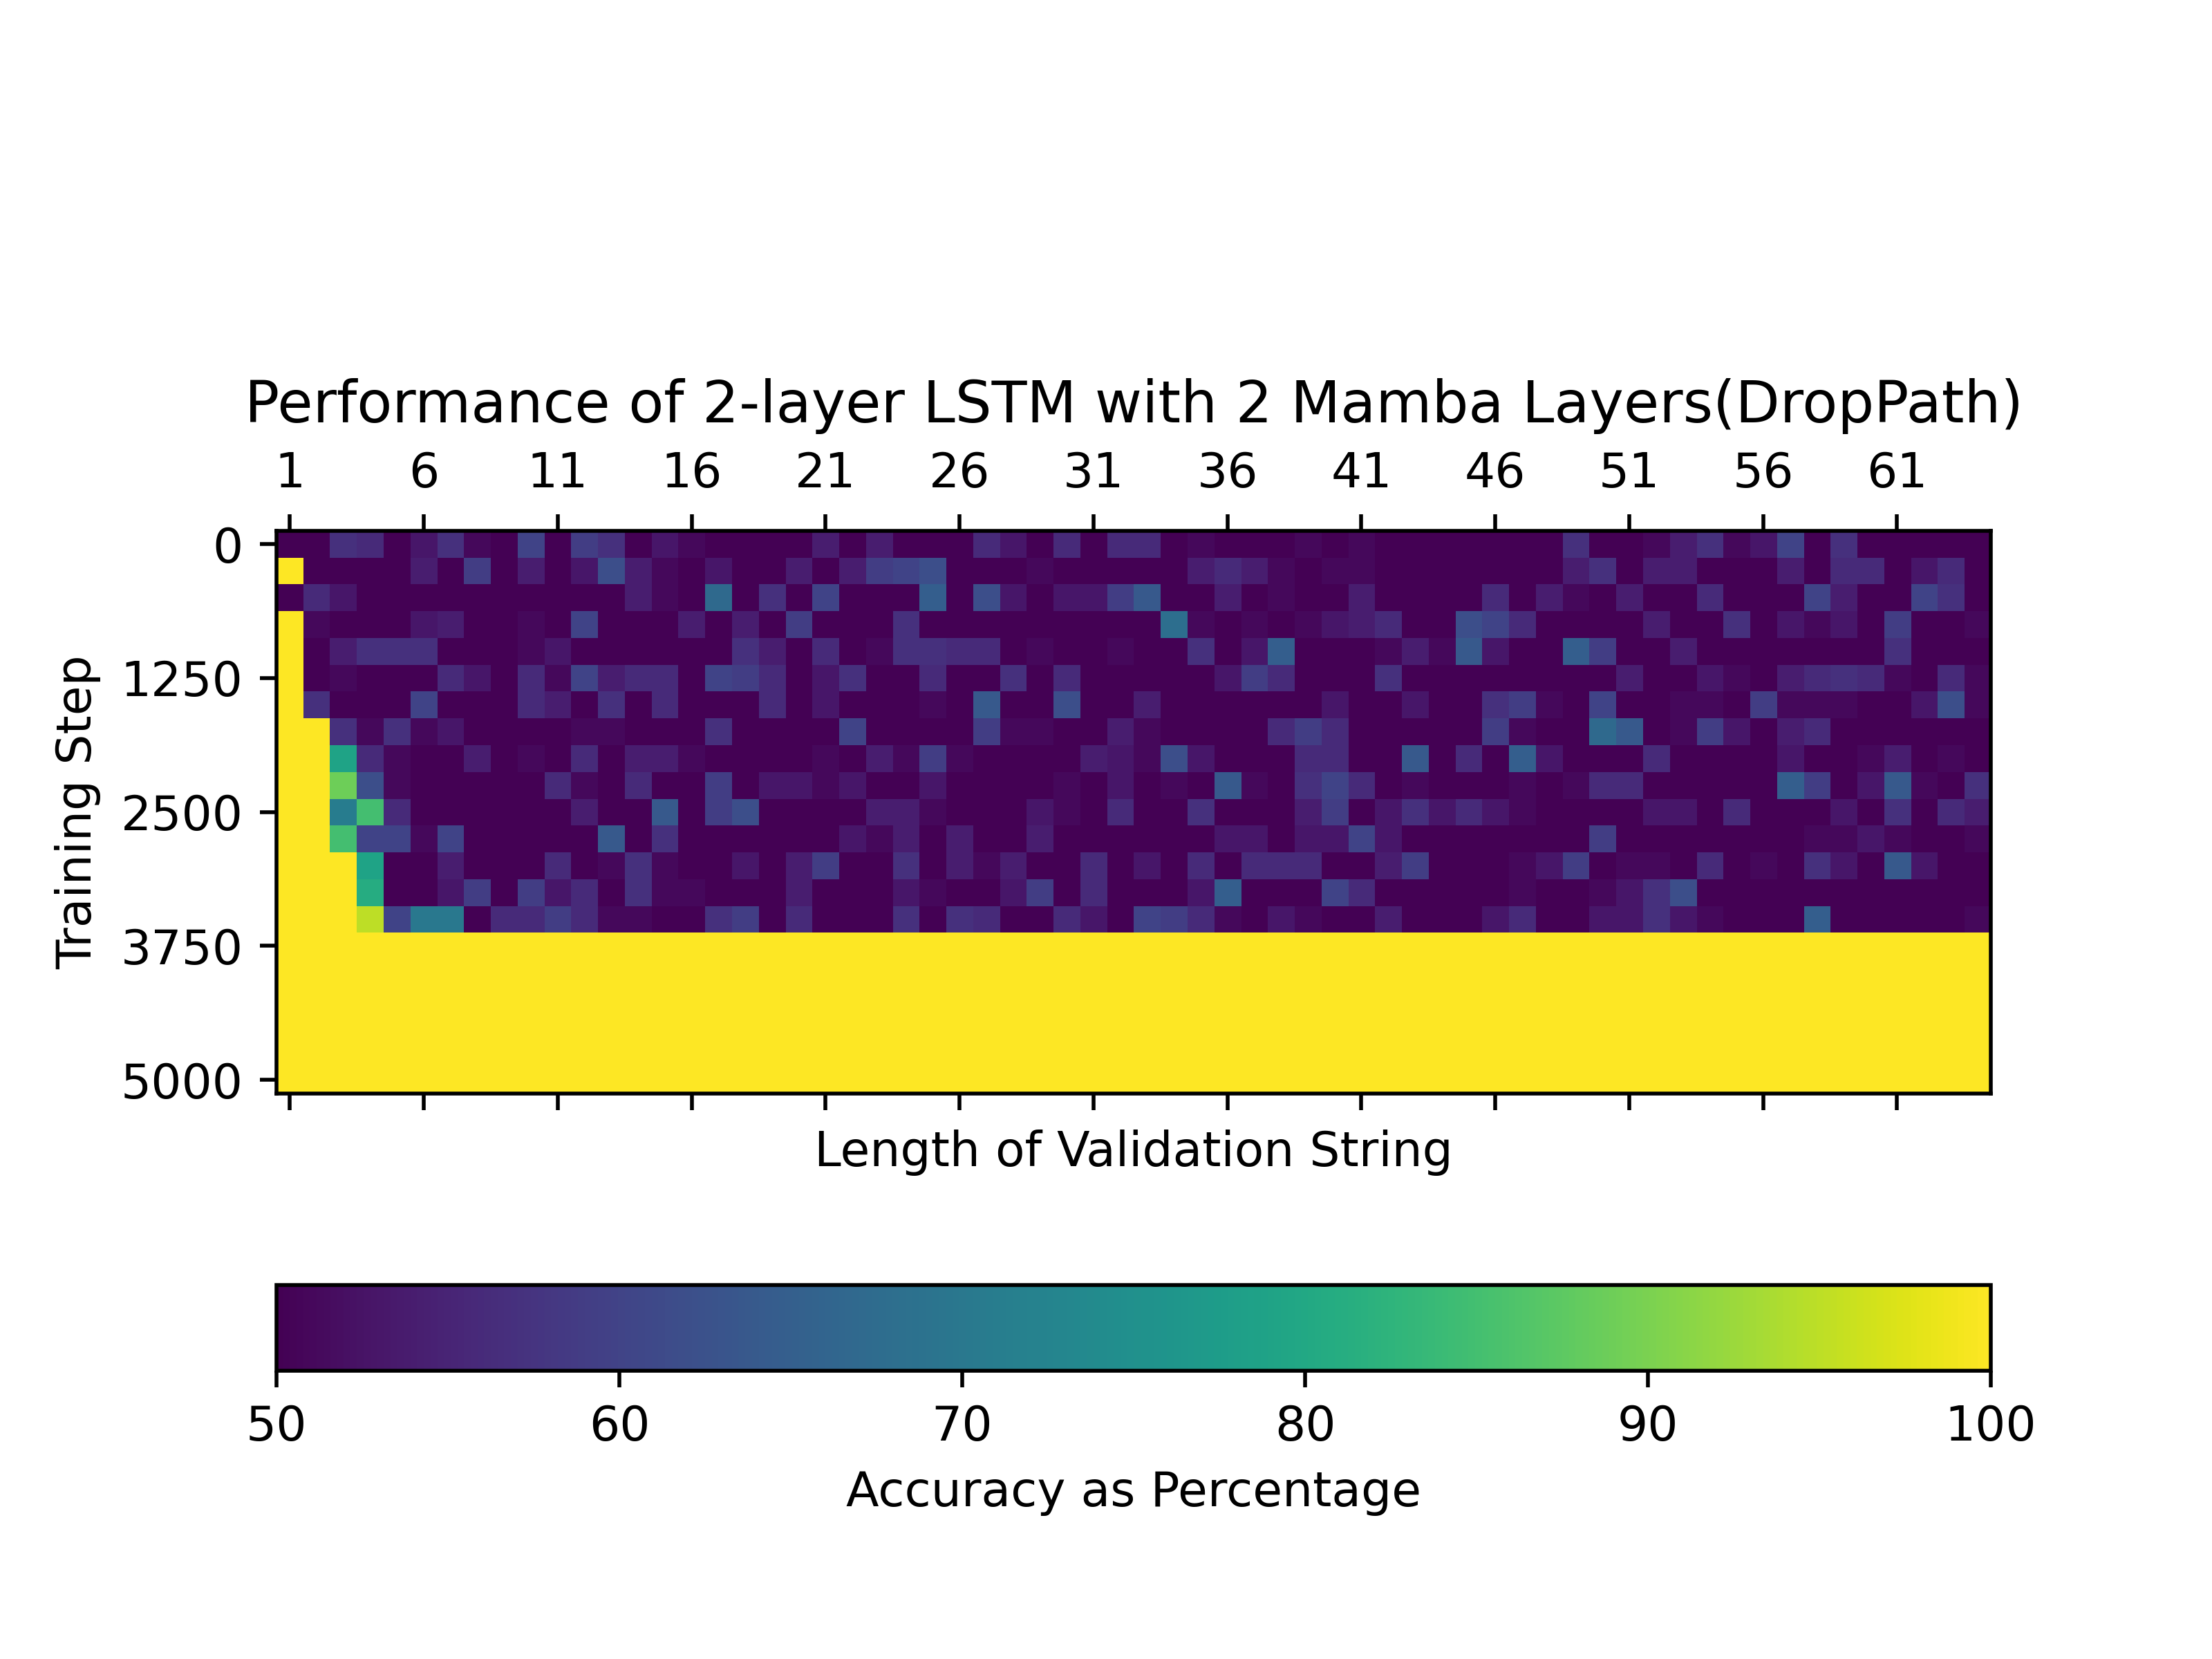
\includegraphics[width=0.8\textwidth]{figures/parity_lstm_True_4_2.png}
        \end{center}
    \end{subfigure}
    \begin{subfigure}{0.5\textwidth}
        \begin{center}
        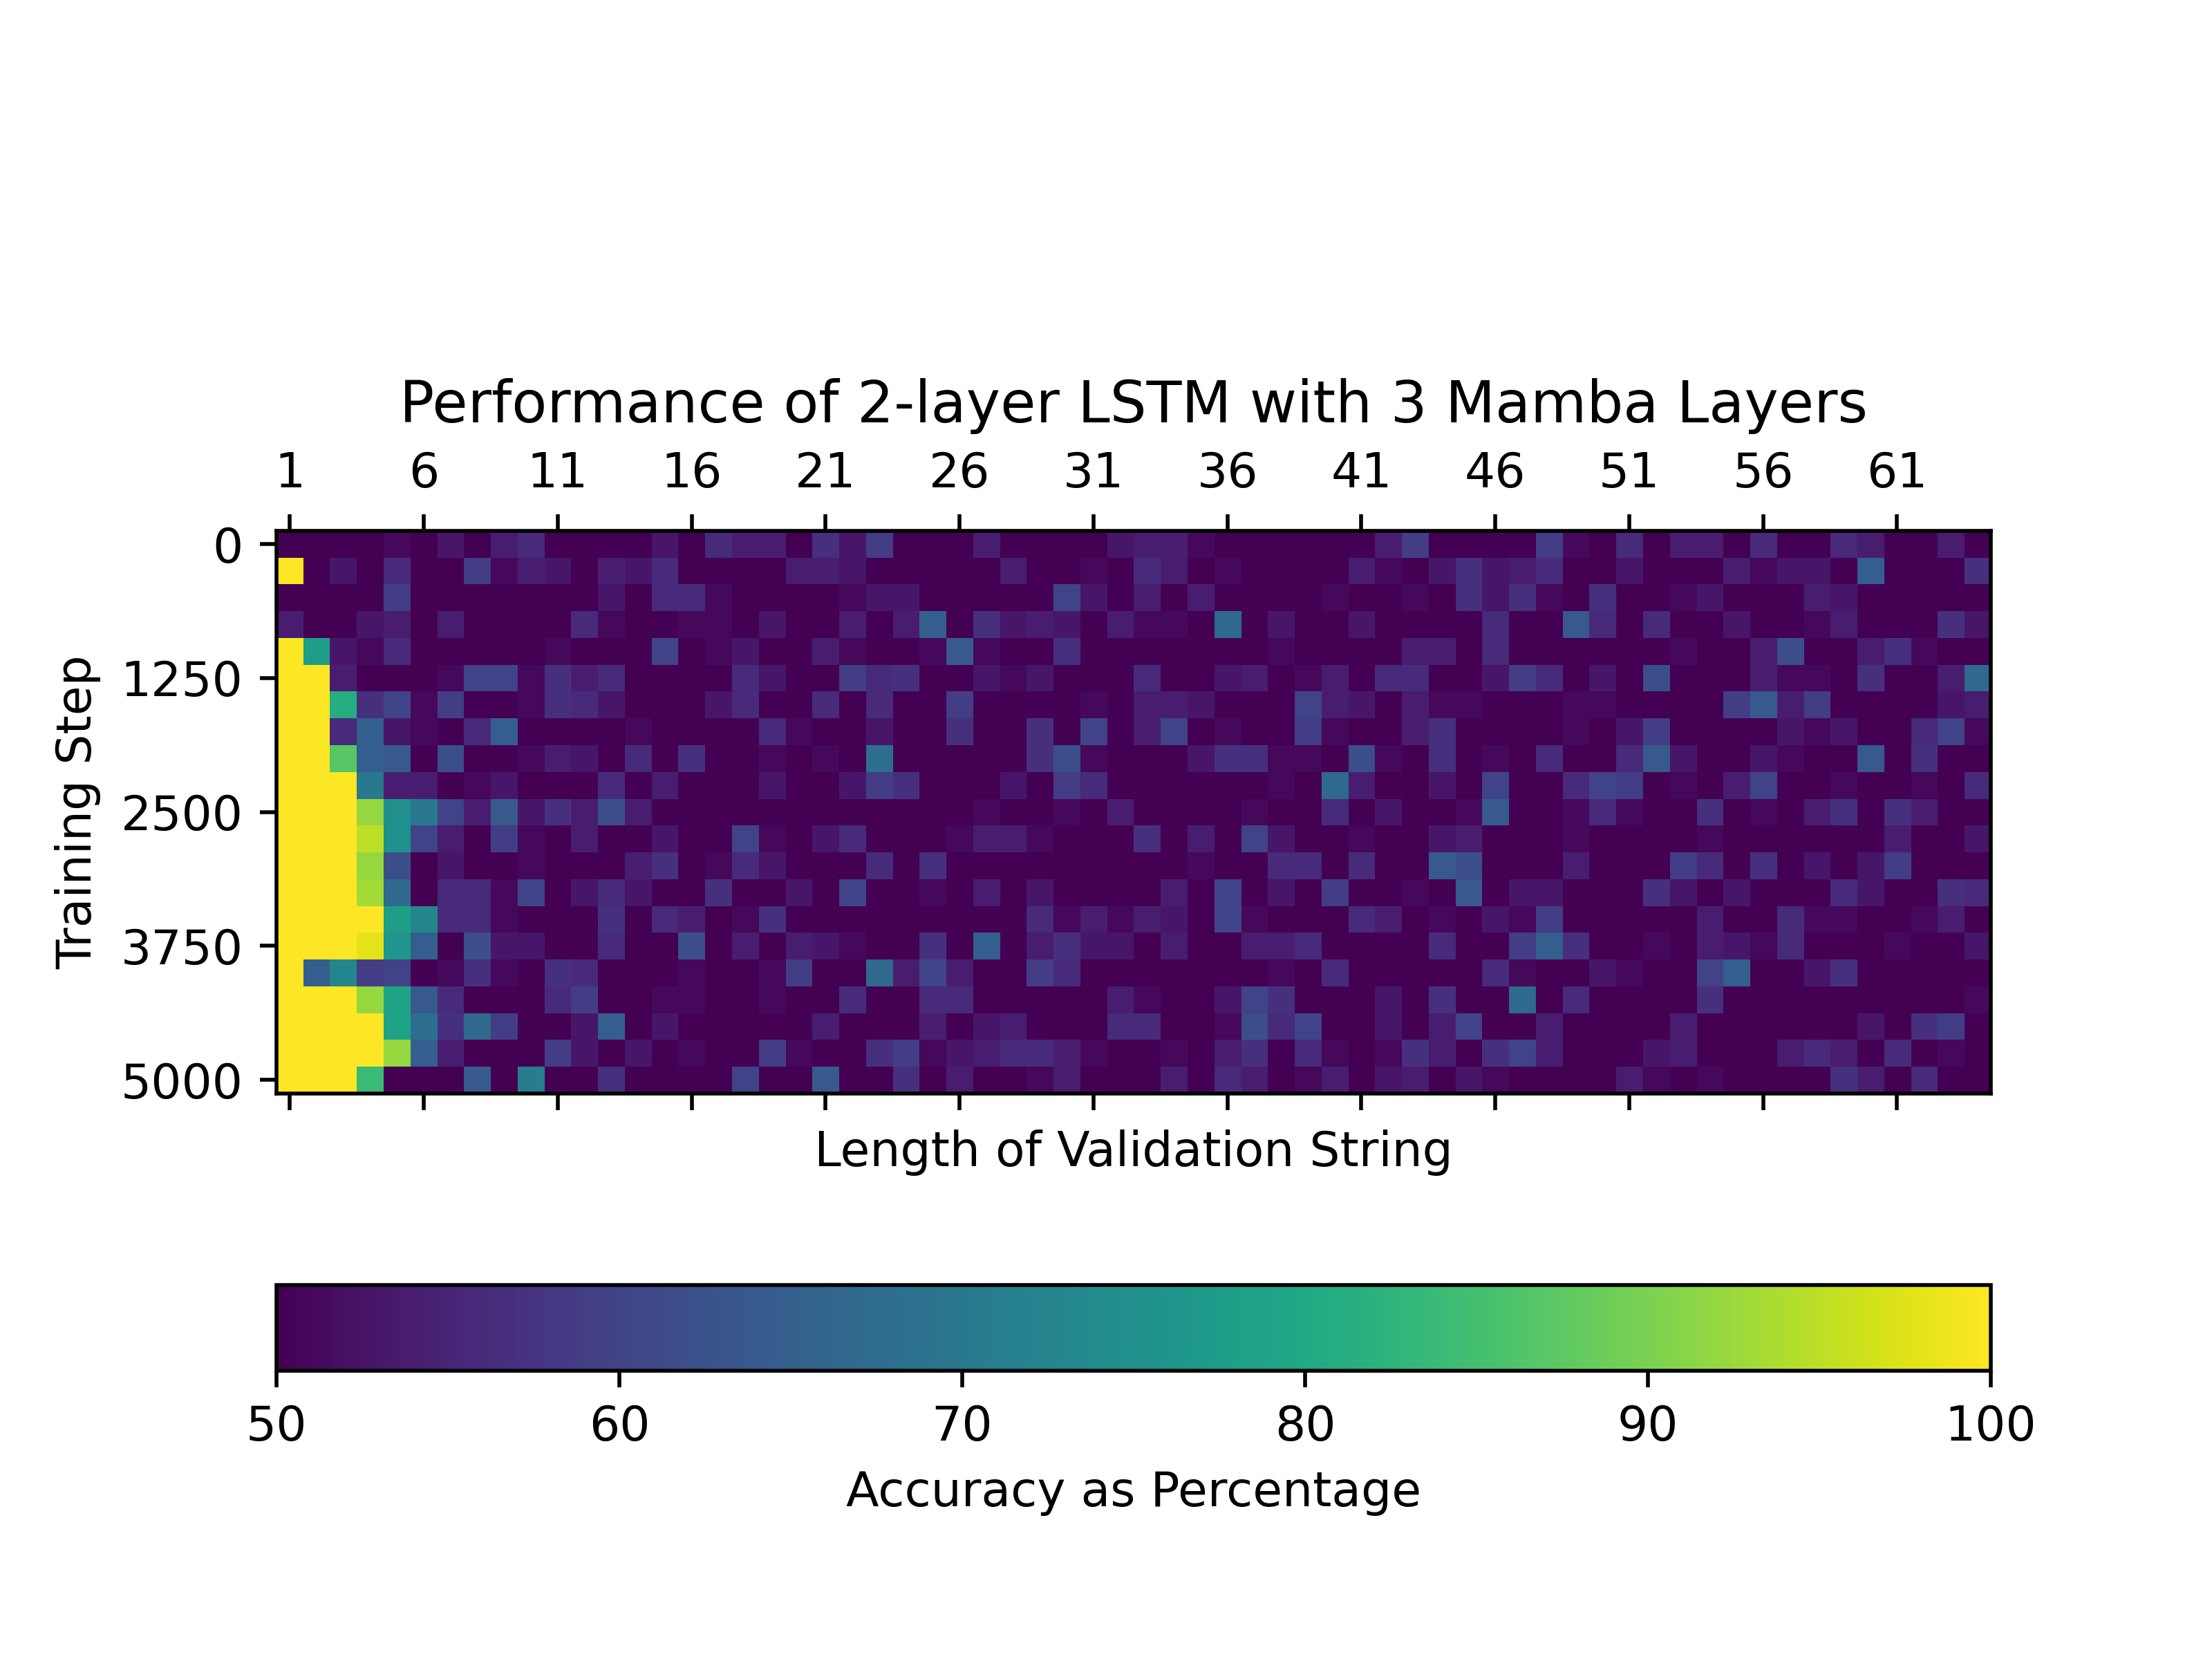
\includegraphics[width=0.8\textwidth]{figures/parity_lstm_False_5_1.png}
        \end{center}
    \end{subfigure}\begin{subfigure}{0.5\textwidth}
        \begin{center}
        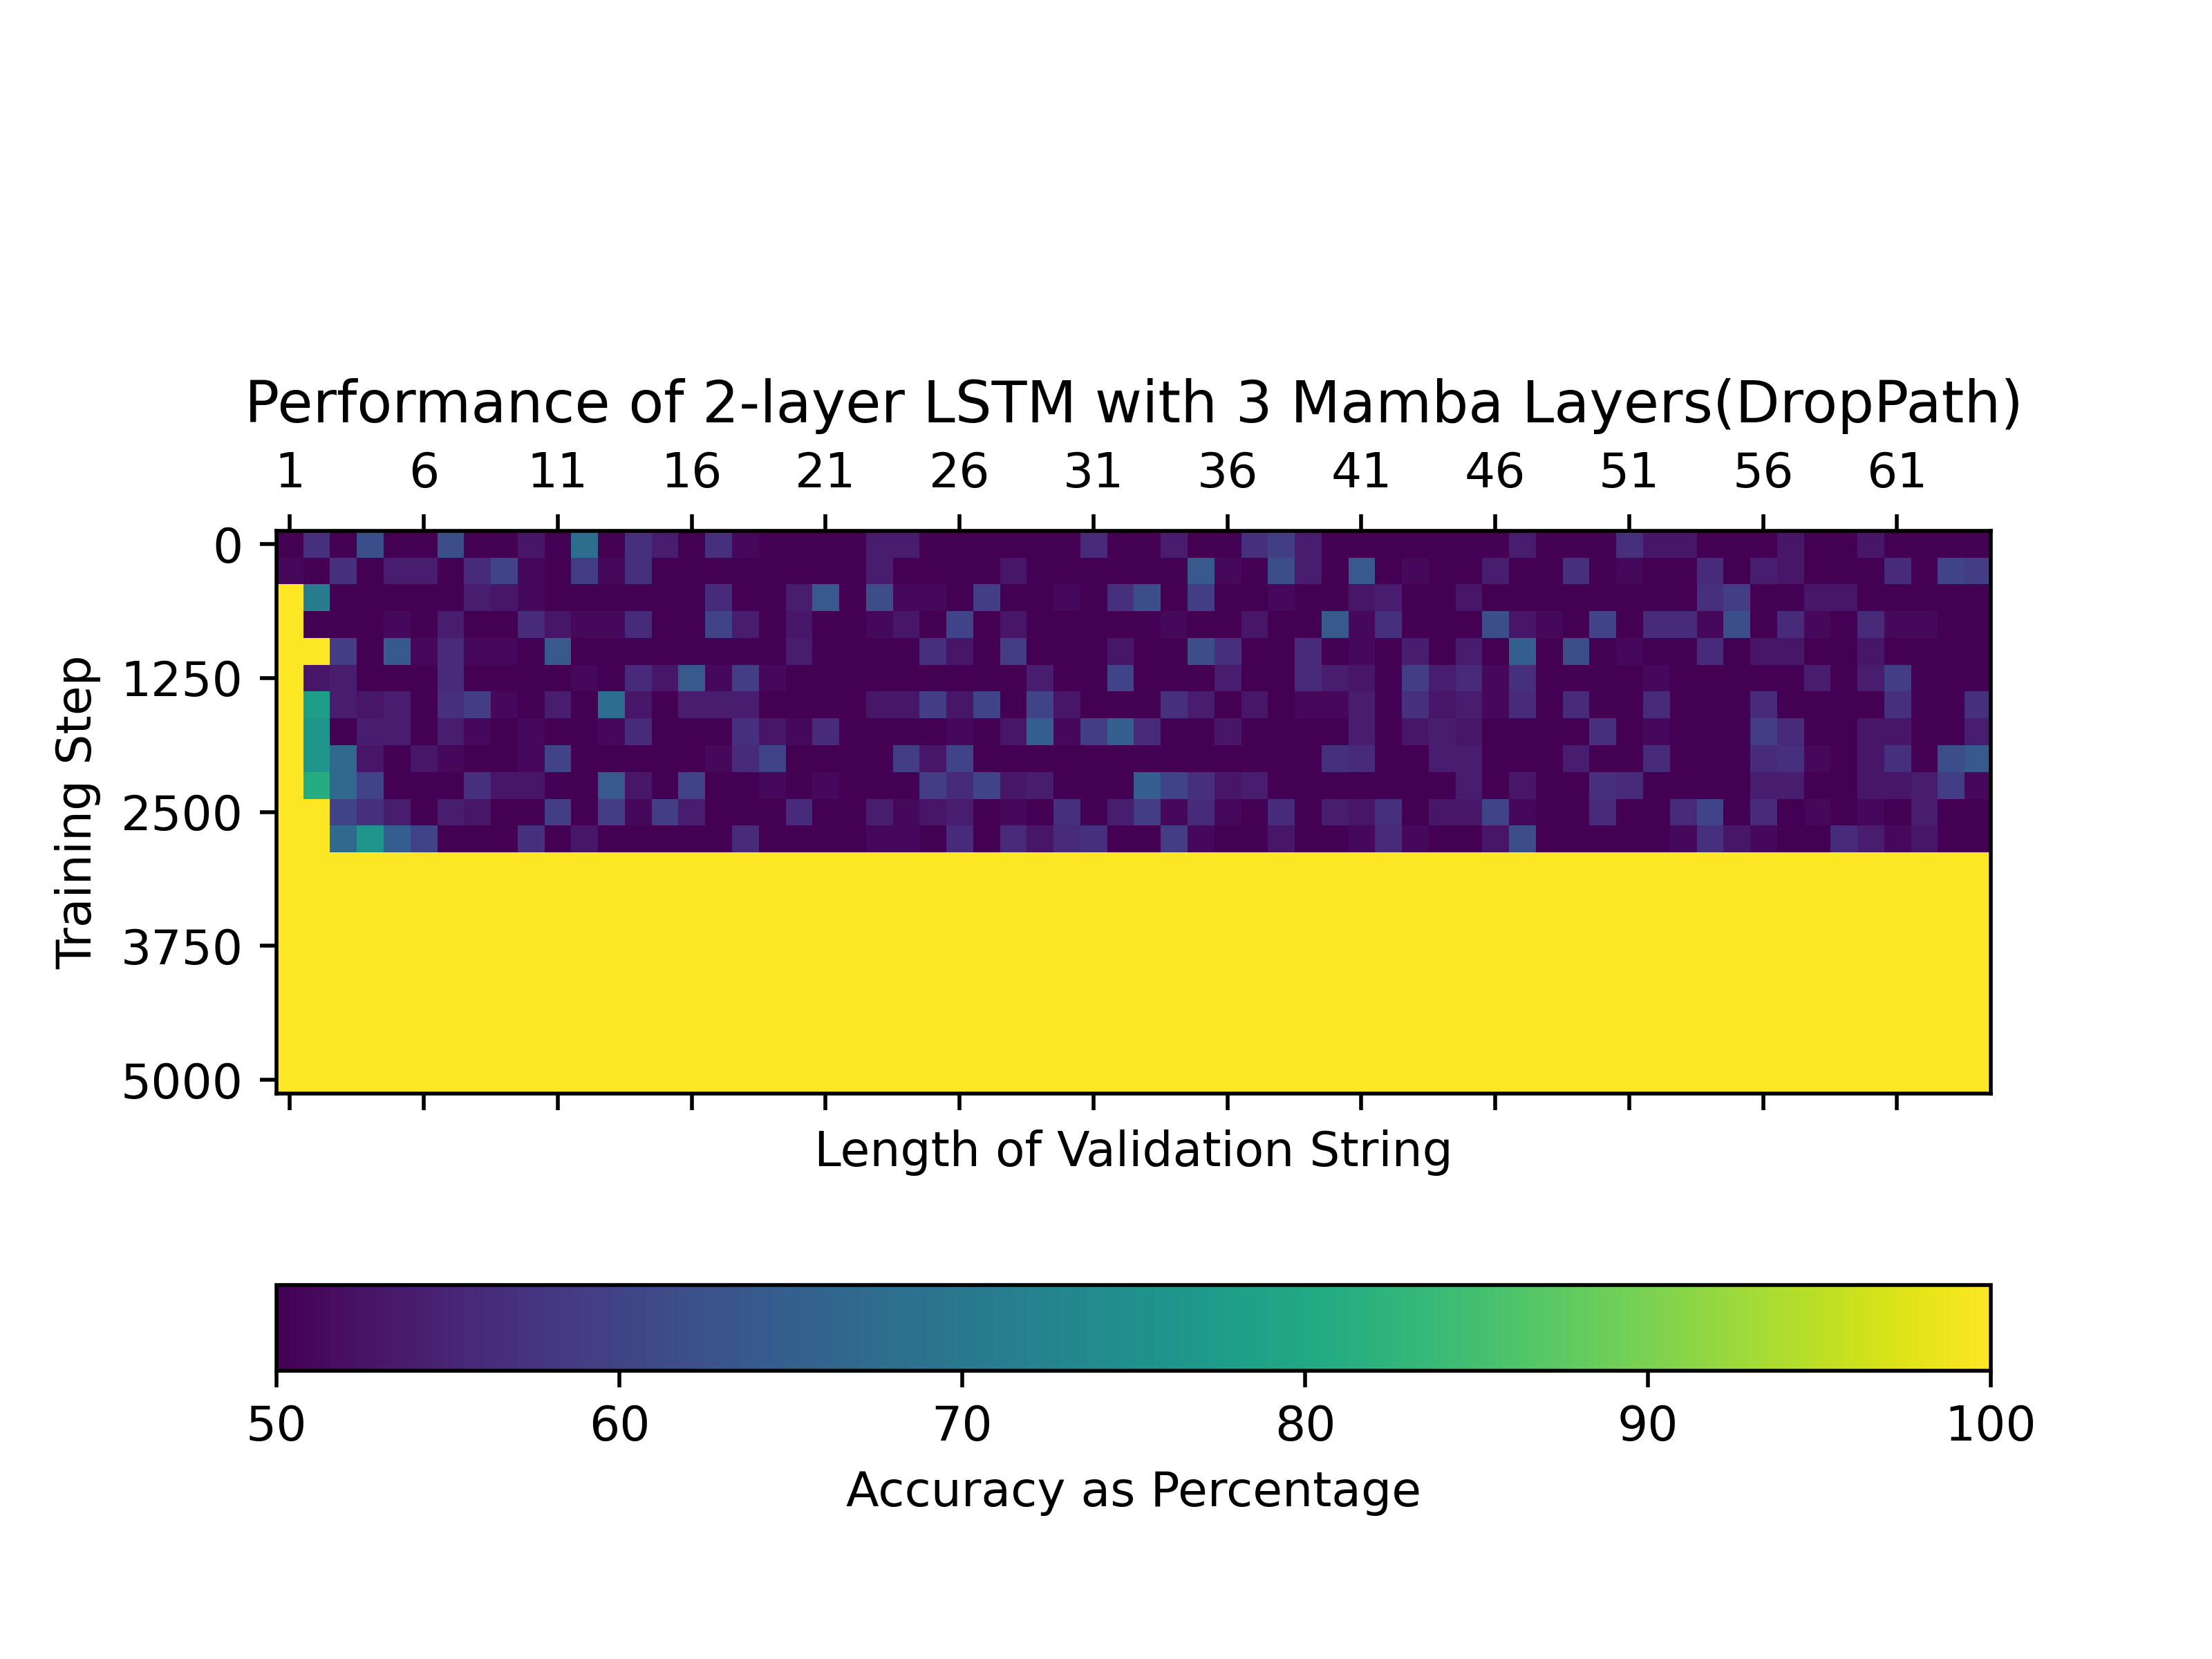
\includegraphics[width=0.8\textwidth]{figures/parity_lstm_True_5_1.png}
        \end{center}
    \end{subfigure}
    \begin{subfigure}{0.5\textwidth}
        \begin{center}
        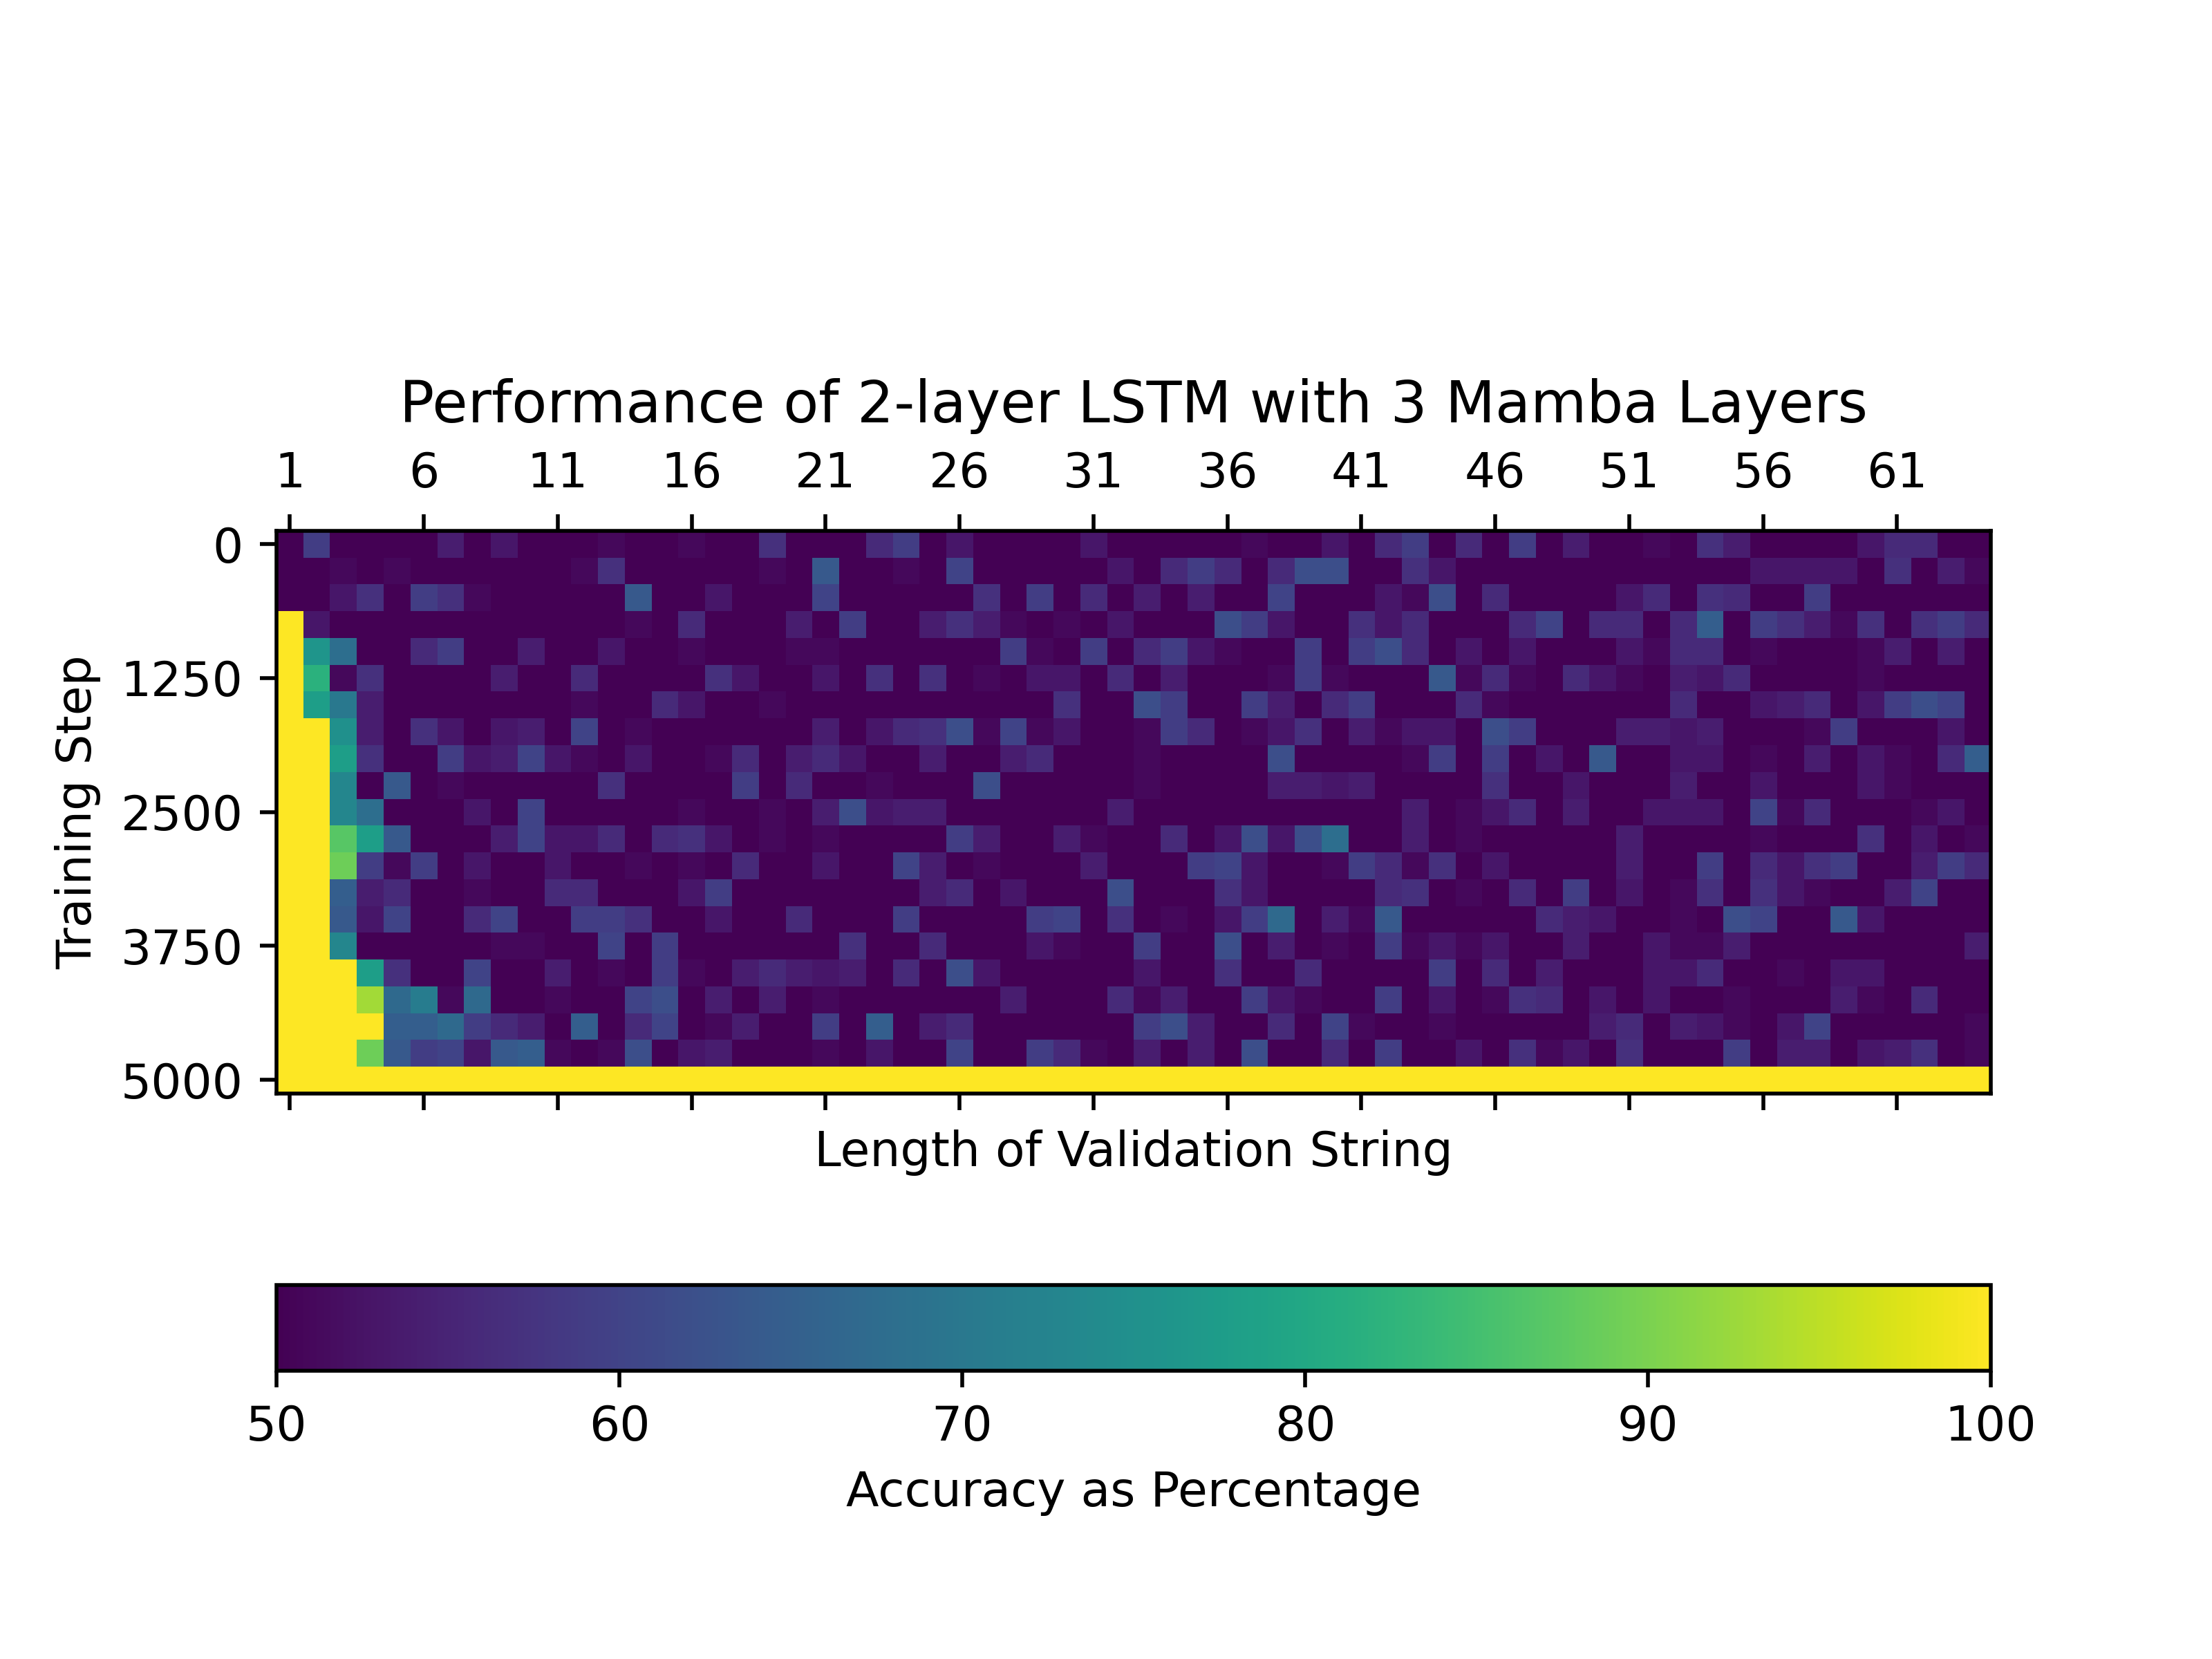
\includegraphics[width=0.8\textwidth]{figures/parity_lstm_False_5_2.png}
        \end{center}
    \end{subfigure}\begin{subfigure}{0.5\textwidth}
        \begin{center}
        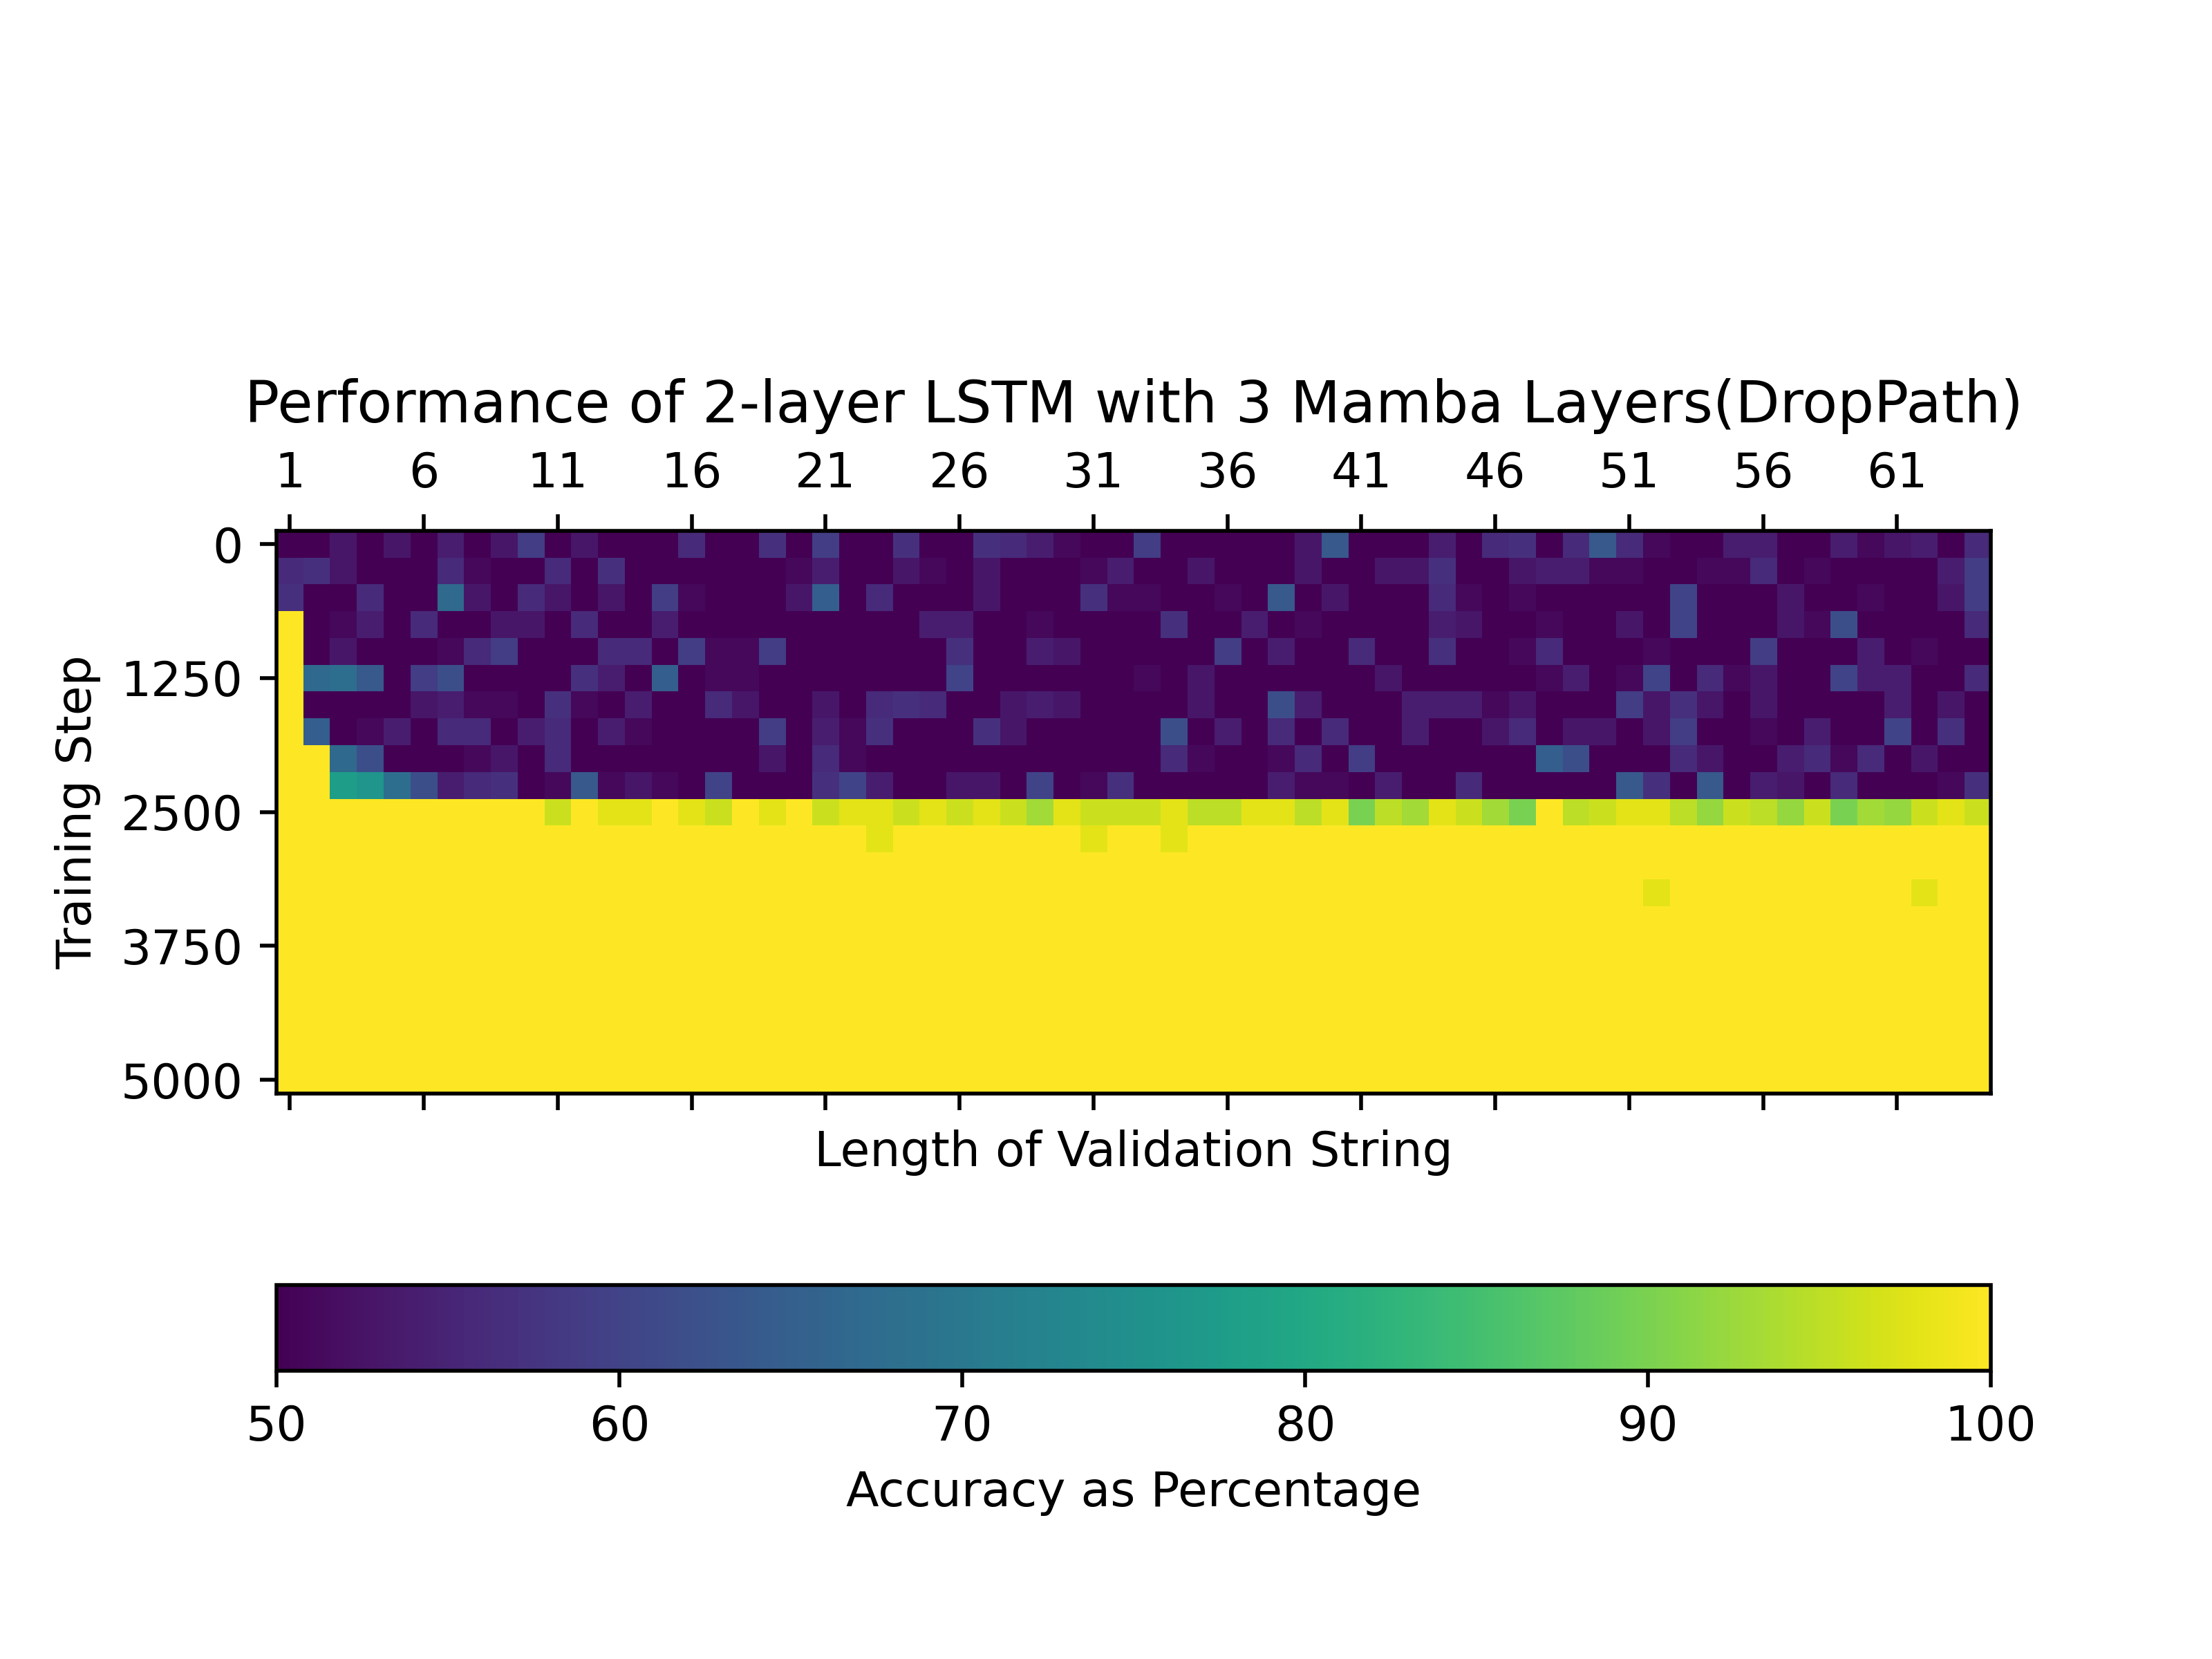
\includegraphics[width=0.8\textwidth]{figures/parity_lstm_True_5_2.png}
        \end{center}
    \end{subfigure}
    \caption{Results for parity}
    \label{droppathresults}
\end{figure}
as shown in Figure \ref{droppathresults}, all of the stacks with droppath
generalized within 5000 training steps, while only 3 of the 6 runs generalized
without drop path.

\subsection{Ability to recognize CFGs}
\begin{figure}
    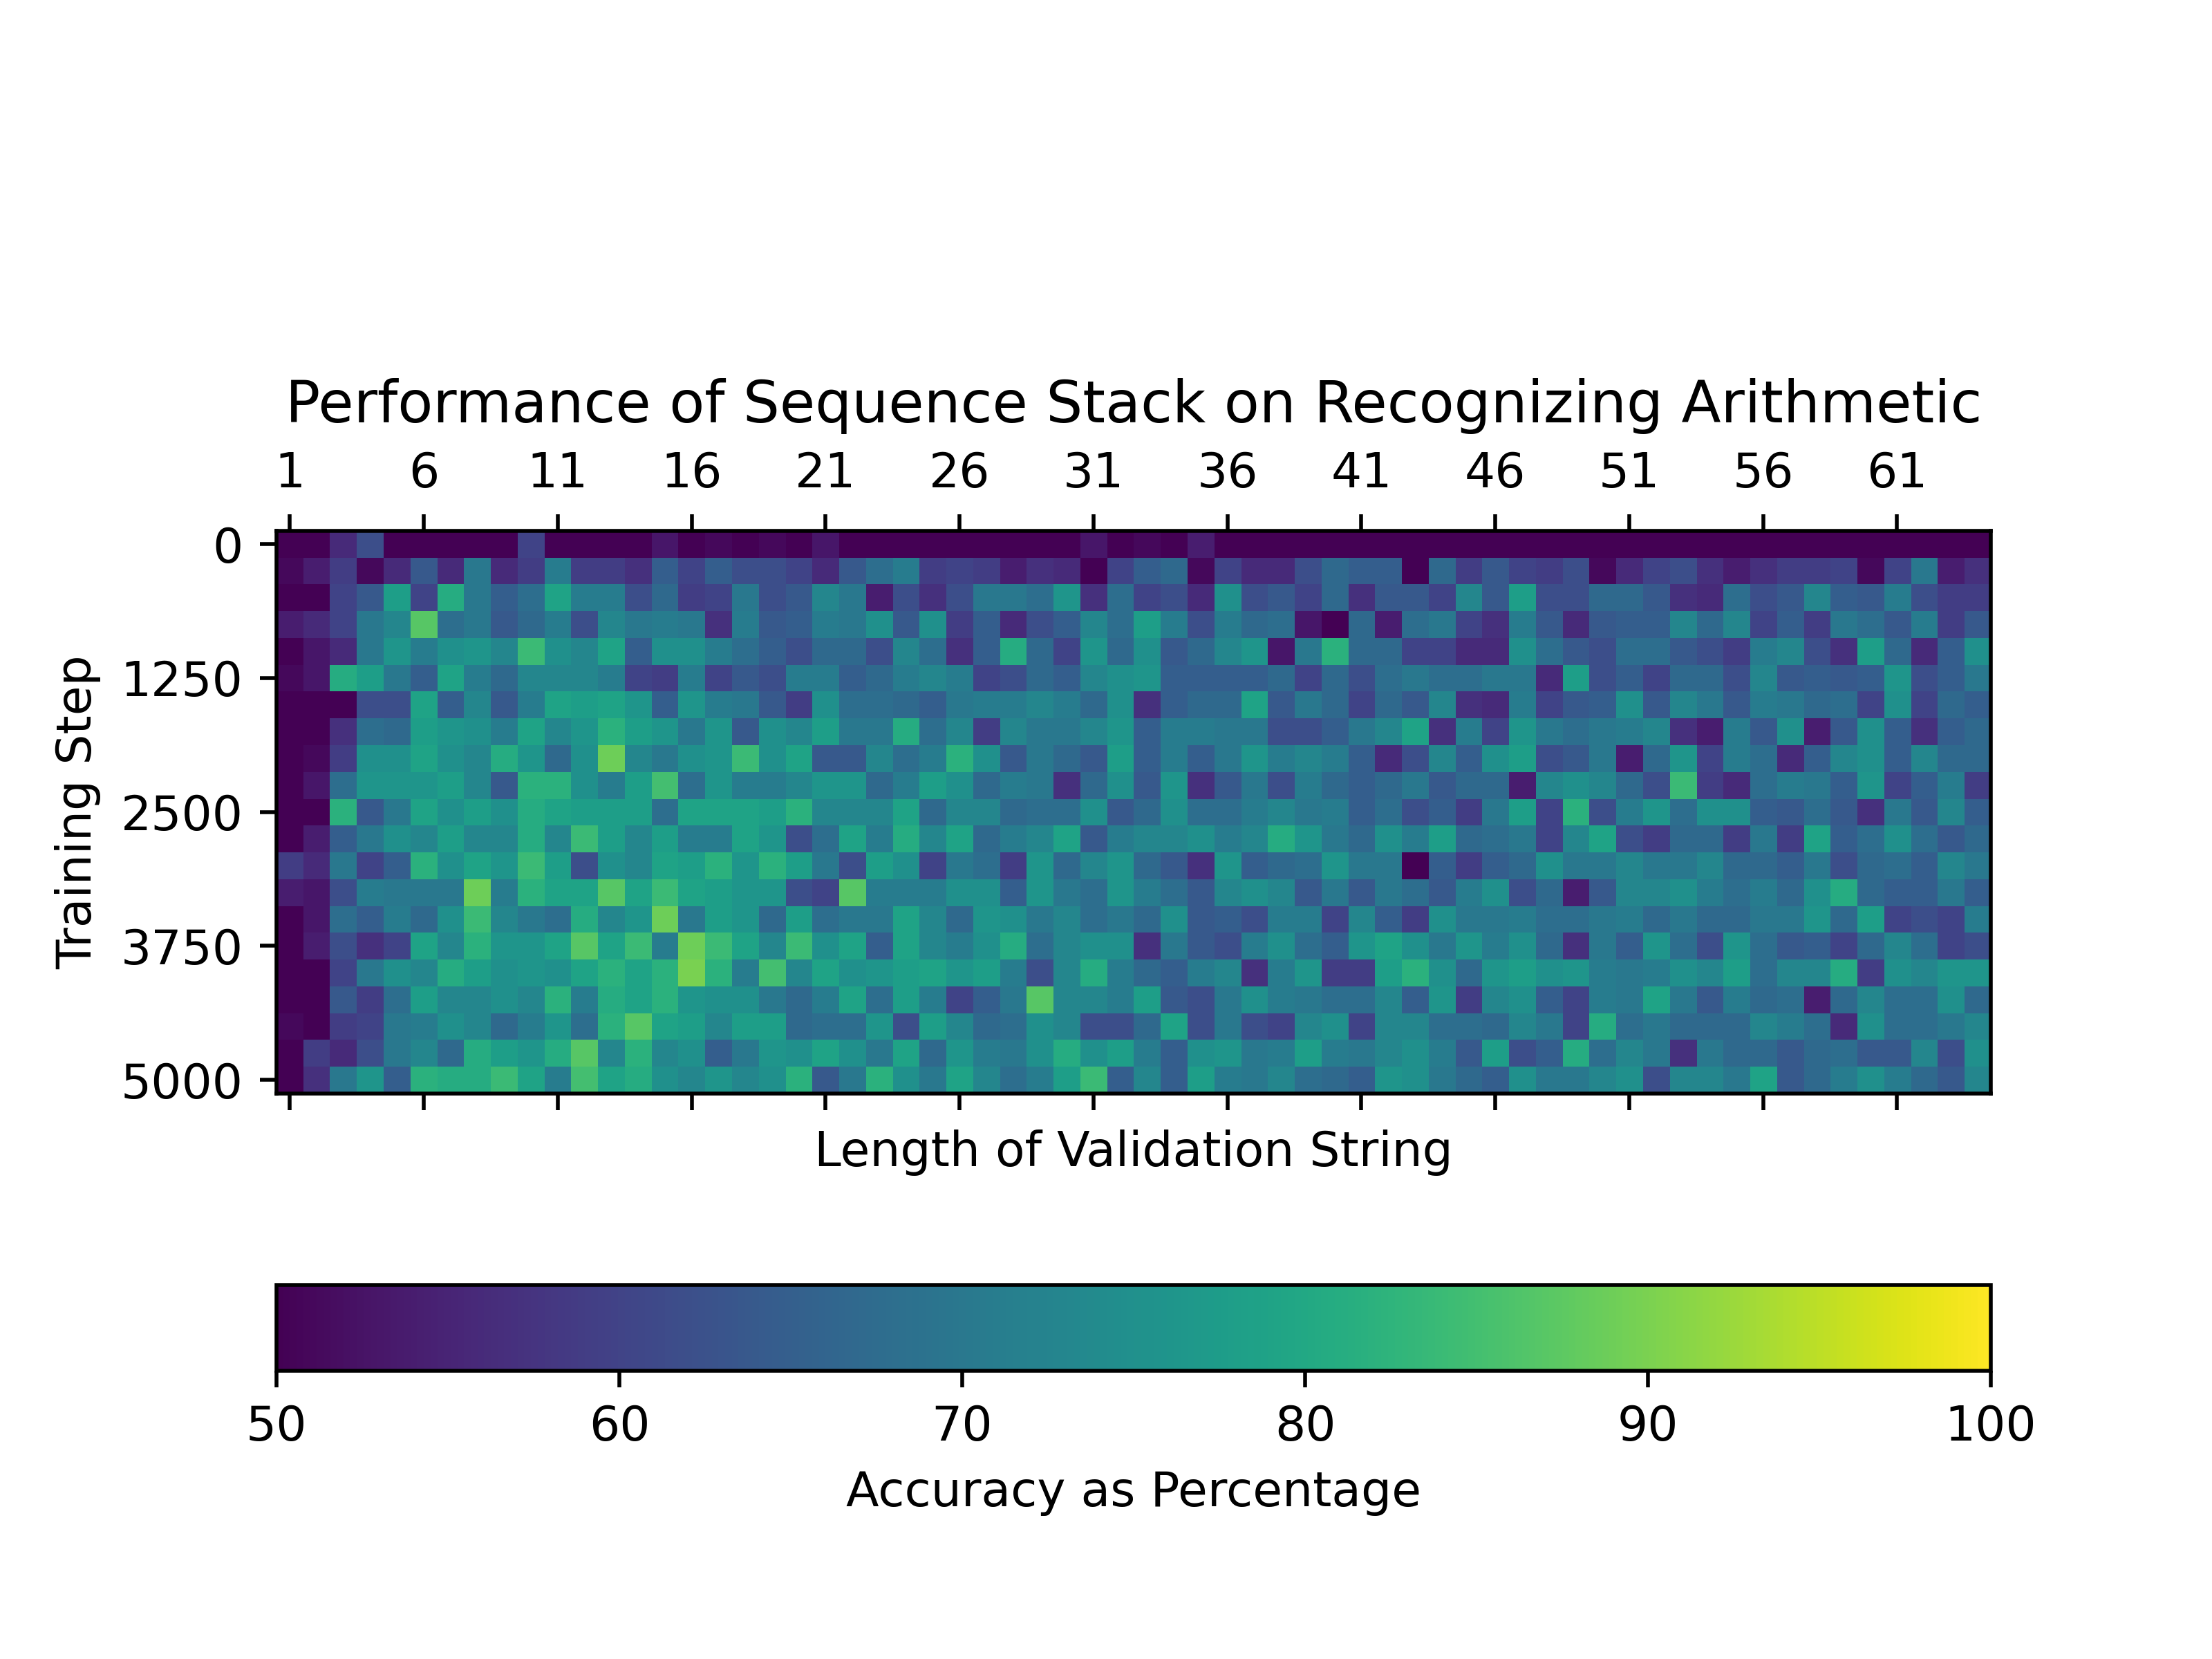
\includegraphics[width=\textwidth]{figures/arithmetic.png}
    \caption{}
    \label{resultsarithmetic}
\end{figure}
An interesting finding from the literature is that despite not being able to
recognize all regular languages, Mamba is theoretically capable of recognizing
some CFGs. For instance, SSMs are theoretically capable of recognizing any Dyck
language by implementing internal counters\cite{ssmformal}.

An important component of many CFG-related operations is matching strings to
non-terminal symbols.
As such, we run the following experiment to test Mamba's ability to learn this
task:

In this experiment, we test the model's ability to recognize nonterminals from
this CFG:
\begin{verbatim}
    G := E
    E := T
    E := E+T
    T := F
    T := T*F
    F := X
    F := (E)
    X := X'
    X := x
\end{verbatim}
This is the CFG for valid arithmetic expressions.
For instance, \verb|(x'+x)*x'| is a valid string in this language while
\verb|x'+x)| is not.

We train a multi-layer Mamba model to distinguish the non-terminal symbols E and
T.
This requires the model to reason about which operations are at the top level
and finding which strings have \verb|+| as a top-level operation.
Since \verb|T| is a subset of \verb|E|, we don't expect the model to perform
perfectly on this task.

\textbf{Model}
The model we use is the same model as in our \texttt{a|bb+} recognizer. We use
the following hyperparameters:
\begin{verbatim}
  mamba_d_model=16
  d_intermediate=16
  mamba_d_state=256
  mamba_d_conv=4
\end{verbatim}

\textbf{Dataset}
The dataset that we use is a synthetic dataset where each instance is generated
as follows:
\begin{itemize}
    \item Choose a random length in the range 1 to 64 inclusive
    \item Choose a random non-terminal: 50\% G, 50\% T
    \item Derive a random string with the given length
\end{itemize}
We generate 5000 batches, with 64 instances per batch.
The sampling step is done efficiently using a dynamic programming algorithm.

\textbf{Results}
As shown in Figure \ref{resultsarithmetic}, the model learns to distinguish the
2 languages with around 70\% accuracy across all string lengths. This is better
than chance and shows that our model is capable of recognizing different
non-terminals.

\subsection{Dyck-1}
\begin{figure}
    \begin{subfigure}{0.5\textwidth}
        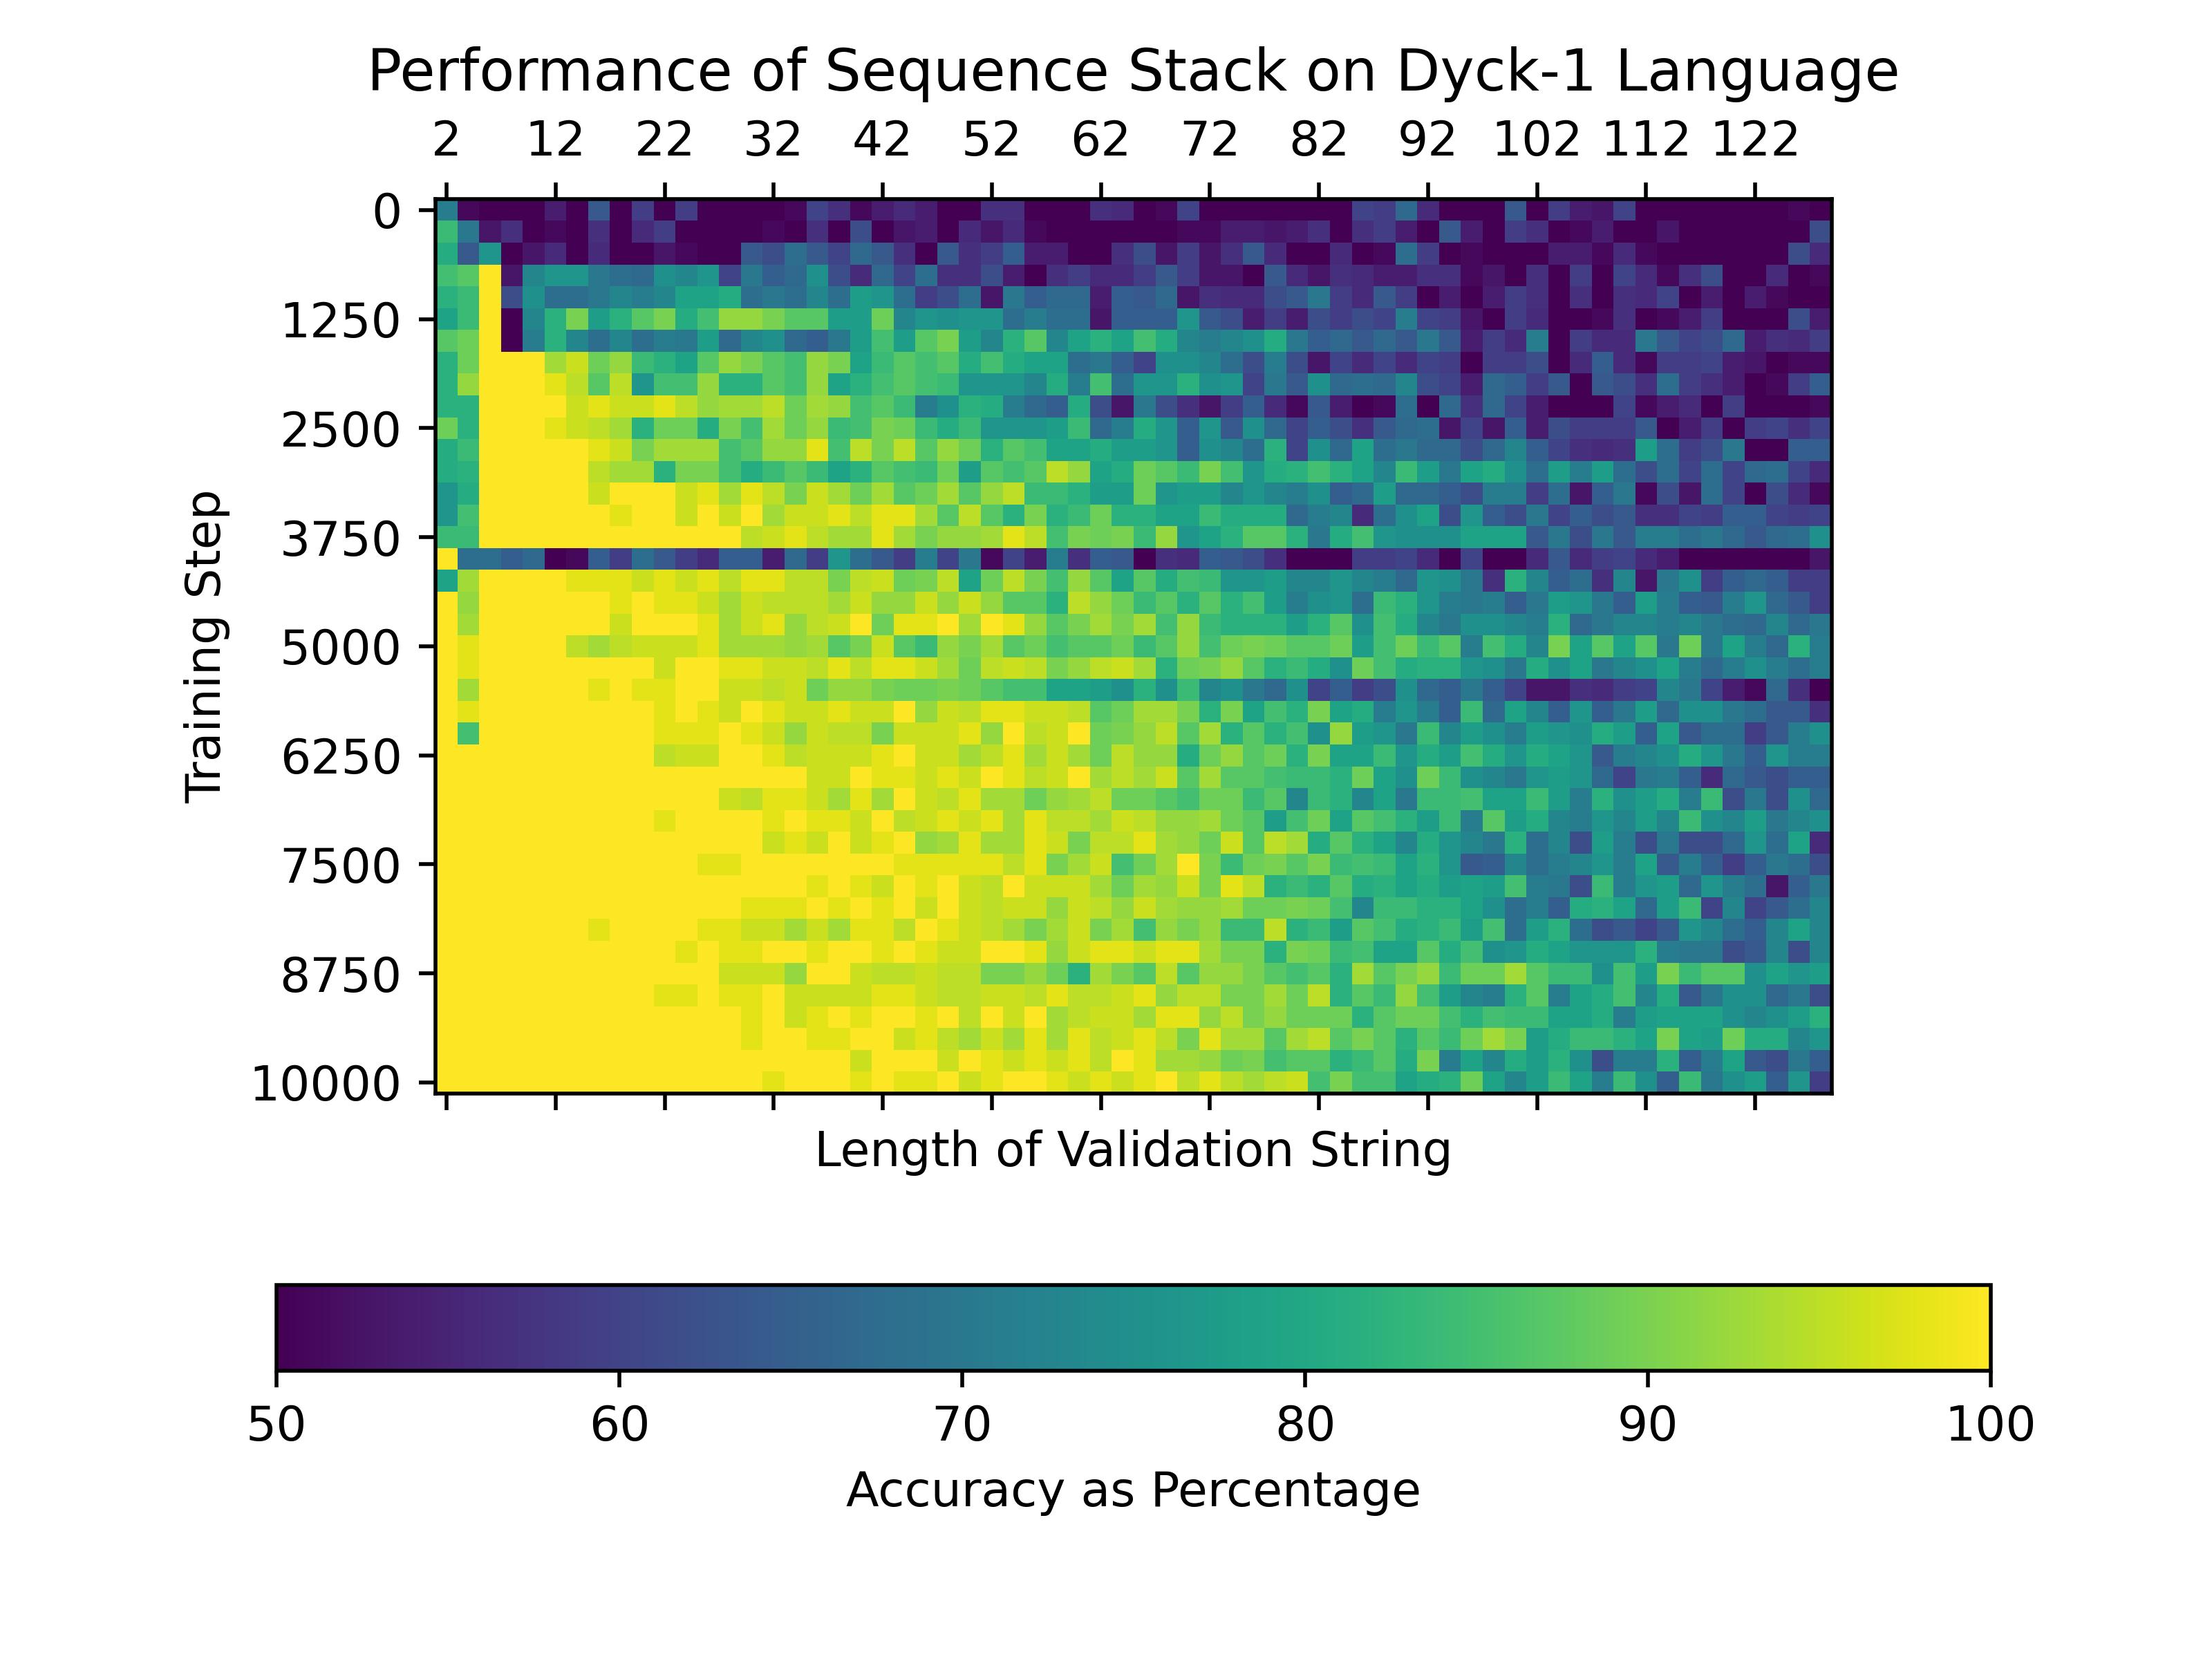
\includegraphics[width=\textwidth]{figures/dyck.png}
        \caption{}
        \label{resultsdyck}
    \end{subfigure}\begin{subfigure}{0.5\textwidth}
        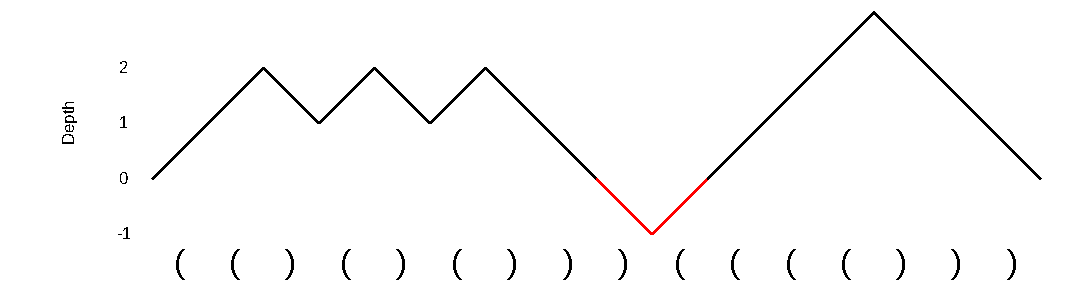
\includegraphics[width=\textwidth]{figures/dyck_challenge.pdf}
        \caption{}
        \label{dyckchallenge}
    \end{subfigure}
    \caption{}
\end{figure}

One specific CFG that is well studied is the Dyck family of languages.
A previous paper\cite{ssmformal} has found that multi-layer Mamba architectures
are theoretically capable of recognizing Dyck-1 instances. In addition, they
claim to experimentally confirm this result. However, they sweep through a set
of hyperparameters such that the largest total state size is many times the
length of their validation samples: in their tests on Dyck-1, their maximum
state size is 256 dimensions while their longest validation string is 100
characters long. In addition, they don't disclose the hyperparameters used to
get achieve the results that they got.
In this section, I reproduce their finding using a much smaller model.

\textbf{Model}
The model that we use is identical to the multilayer Mamba model described in
the first experiment.
The hyperparameters that we use are:
\begin{verbatim}
  n_layer=2
  d_intermediate=64
  mamba_d_model=4
  mamba_d_state=2
  mamba_d_conv=2
\end{verbatim}
The total state dimension is given by
$$
n_{layer} * d_{model} * (d_{state} + d_{conv} - 1) = 24
$$

\textbf{Dataset}
The dataset that we use to train the model is an even split between Dyck-1
instances and "difficult" non-instances(explained in the next paragraph).
The method for generating instances here is essentially the same as in the
previous sections:
\begin{itemize}
    \item The string lengths are uniformly chosen from the set
        $[2, 64] \cap 2\ZZ$($[2, 128] \cap 2\ZZ$ for the validation set).
    \item The class is randomly chosen: there is a 50\% likelihood that we
        choose a Dyck-1 string, and a 50\% likelihood that we choose a hard
        non-Dyck-1 string.
    \item Within these constraints, we take a roughly\footnote{
        The sampling algorithm for hard non-Dyck-1 strings is not perfectly
        uniform, although we don't expect the non-uniformity to significantly
        affect our results.
    } uniform sample of strings within this pair of constraints.

\end{itemize}
We generate 10000 batches with 64 instances per batch. The validation set has
lengths samples from $[2, 128] \cap 2\ZZ$ instead of $[2, 64] \cap 2\ZZ$ so that
the model is tested on unseen data.

To explain what hard non-instances are, it's first important to understand the
rules for valid Dyck-1 strings.
Dyck-1 strings are equivalent to matched strings of parentheses.
The validity of a string can be calculated by scanning along the string and
tracking the "depth" at each character. The character \verb|(| increases the
depth, since it enters a pair. The character \verb|)| decreases the depth, since
it exits a pair.
If the depth is never negative, and the final depth is 0, then the string is
valid.
A difficult string ends at a depth of 0, and only has a negative depth of -1 at
one point near the middle.
This ensures that any counter-based recognizer needs to be numerically precise,
since a small error can prevent the model from recognizing the small negative
region.
An example of such a string is shown in Figure \ref{dyckchallenge}

\textbf{Results}
As shown in Figure \ref{resultsdyck}, the smaller model is able to achieve
better-than-chance results on strings twice the length of its training data.
In addition, these strings are significantly larger than the maximum theoretical
state dimension($128 > 24$).
This is a strong piece of evidence that the model is using a depth counter to
evaluate string membership.

\subsection{Conclusion of Exploratory Section}
In these mini-experiments, we've learned some features of Mamba that will be
useful for model design.
We've learned that the Mamba architecture has a strong inductive bias for
fixed pattern-matching.
This is a promising result, since OCR is closely related to pattern-matching.
In fact classical OCR algorithms have used pattern matching for both character
recognition and context-based
correction\cite{classicalocr,classicalocrincontext}.
We also learned that the Mamba architecture tends to perform better with gating
and other mechanisms to isolate it from the rest of the model. As such, we will
include drop-path in our model design when its mixed with other layer types.
Finally, although not useful to our own endeavors, we've also confirmed an
interesting theoretical result about Mamba's expressive capacity.
